\documentclass[11pt]{report}
\usepackage[utf8]{inputenc} 
\usepackage[backend=bibtex, maxnames=3, bibencoding=utf8, sorting=none]{biblatex}
\usepackage[T1]{fontenc}
\usepackage[english]{babel}  
\usepackage[pdftex]{graphicx}
\usepackage[titles]{tocloft}
\usepackage{amsthm}
\usepackage{amsmath}
\usepackage{amssymb}
\usepackage{mathrsfs} 
\usepackage{enumitem}
\usepackage[babel=true]{csquotes}
\usepackage{wrapfig}
\usepackage[right=1.25in,left=1.25in,top=1.in,bottom=1.in]{geometry}  %% right=0.75in,left=0.75in,top=0.75in,bottom=0.75in
%\usepackage{etoolbox}
\usepackage[toc,page]{appendix}
\usepackage{caption}
%\usepackage{captionof}
\usepackage{pdfpages}
\usepackage{titlesec}
%\usepackage{fancyhdr}
%\usepackage[nottoc]{tocbibind}
\usepackage{fancyhdr,lastpage}
\usepackage{array}
% \usepackage{eurosym}
\usepackage[hidelinks]{hyperref}
\usepackage{todonotes}
\usepackage{lipsum}
\usepackage{svg}
\usepackage{newunicodechar}
\usepackage{gensymb}
\usepackage{booktabs}

% \DeclareUnicodeCharacter{176}{°}
% \DeclareUnicodeCharacter{9702}{°}

\bibliography{PDM_references.bib}
% \bibliographystyle{unsrt}

\graphicspath{{../figures/}}
\titleformat{\chapter}[hang]{\normalfont\huge\bfseries}{\thechapter.}{20pt}{\huge}

\title{Spherical Convolutional Neural Networks}
\author{Frédérick Matthieu Gusset}

\makeatletter
\let\thetitle\@title
\let\theauthor\@author
\makeatother

\DeclareMathSizes{10}{11}{8}{8}   % Pour un texte de taille 10 
\titlespacing*{\chapter} {0pt}{15pt}{15pt}
\makeatletter
\patchcmd{\printbibliography}{%
 \chapter*{\bibname}\@mkboth{\MakeUppercase\bibname}{\MakeUppercase\bibname}}{%
 \chapter{References}}{}{}
\makeatother

\renewcommand{\headrulewidth}{0pt}
\renewcommand{\footrulewidth}{0.4pt}

\headheight 14pt
\fancypagestyle{plain}
{
  \fancyfoot[L]{F. Gusset}% Left footer
	\fancyfoot[C]{}
  \fancyfoot[R]{\thepage}% Right footer
  \fancyhead[L]{}
}
\pagestyle{plain}% Set page style to plain.

\setlength{\cftbeforechapskip}{0pt}  %enlève espace entre chapitre dans sommaire
\newcolumntype{C}[1]{>{\centering\arraybackslash }b{#1}}

\setlength{\parindent}{1em}

\begin{document}
% \nocite{*}
\thispagestyle{empty}
\begin{center}
    \vspace*{0.9 cm}
    %\includegraphics[scale = 0.8]{EPFL-Logo-RVB-55.jpg}\\[0.5 cm]	% University Logo
    %
	%\textsc{MICRO-498}\\[0.5 cm]
    
% 	[0.4 cm]
    \vspace{7pt}
	{\large % Course Code
	\textsc{Projet de Master - 2019 - Section de Microtechnique\\[1 cm]~}\\[1 cm]				% Course Name 
    }
    % 
\includegraphics[width=0.6\linewidth]{figures/EPFL_Logo_Digital_RGB_PROD.png}
	\rule{\linewidth}{0.2 mm} \\[1 cm]
	{\huge \bfseries \thetitle}\\
    \vspace{10pt}
    { \large \bfseries Empirical analysis of SCNNs }
    \vspace{10pt}%\\
    
	\rule{\linewidth}{0.2 mm} \\[1 cm]
	
	
    %\\[1 cm]
    \textsc{\bfseries Fr\'ed\'erick Matthieu Gusset}
	\\[1.7 cm]
	
	\begin{minipage}{0.1\textwidth}
		\begin{flushleft} \large
			\textsc{}\\
            \vspace{10pt}
            \textsc{} \\
			\vspace{10pt}
			\end{flushleft}
			\end{minipage}~
		\begin{minipage}{0.3\textwidth}
		\begin{flushleft} \large
			\textsc{Professor}\\
            \vspace{10pt}
            \textsc{Supervisors} \\
			\vspace{10pt}
			\end{flushleft}
			\end{minipage}~
			\begin{minipage}{0.4\textwidth}
			\begin{flushright} 
			\vspace{10pt}\large
			\textsc{Pierre Vandergheynst}\\
            \vspace{10pt}
			\textsc{Michaël Defferrard}\\
			\textsc{Nathanaël Perraudin}
		\end{flushright}
	\end{minipage}\\[2 cm]
	
	{\large % Course Code
	\textsc{LTS2\\[1 cm]~}\\[1 cm]				% Course Name 
    }
	
	\vfill~
	
	\textsc{\today} \\[2 cm]
\end{center}

\cleardoublepage
\thispagestyle{empty}
\mbox{~}
\cleardoublepage
% \thispagestyle{empty}
% \begin{center}
% \textbf{Spherical Convolutional Neural Networks}
% \end{center}
% \paragraph*{}
% In the last 5 years, the field of Machine Learning has been revolutionized by the success of Deep Learning. Thanks to the increasing availability of data and computations, we now are able to train very complex and deep models to solve challenging tasks better than we ever did.
% \paragraph*{}
% Nevertheless, Deep Learning is successful when the network architecture exploits properties of the data, allowing efficient and principled learning. For example, convolutional neural networks (CNNs) revolutionized computer vision because the network architecture has been specifically designed to deal with images. The main characteristic of CNNs is to be equivariant to translation: if the input is translated, so is the output. The translation equivariance property is extremely valuable in dense tasks such as segmentation. For global tasks such as object recognition, translation invariance is sought: a translation of the input image should not result in a change of class. This property of images and the adapted CNN architecture enables the spatial sharing of weights that dramatically reduces the number of parameters to be learned. By exploiting translation equivariance, CNNs exhibit lower computational and learning complexities on data that satisfies this property.
% \paragraph*{}
% Beyond images, we need architectures adapted to other kinds of data, encoding both domain specific knowledge and data specific characteristics. For instance, spherical data is very common in (i) climate science with data on the Earth, (ii) in cosmology, where most observations are made from the Earth (see Figure 1), and (iii) in virtual reality, where one often works with user-centered 360\degree images. Spherical data is represented by pixels that live on the sphere. They are like curved images, but without borders and a potentially arbitrary orientation. Similarly to images, we’d like our architectures to exploit properties of the spherical domain. Instead of translation, the spherical domain naturally suggests equivariance to the rotation group SO(3): a rotation of the input implies the same rotation of the output.
% \paragraph*{}
% Figure 1: Example maps on the sphere: (left) the cosmic microwave background (CMB) temperature map from Plank, (middle) map of galaxy number counts, and (right) simulated weak lensing convergence map.
% \paragraph*{}
% So far, two approaches have been followed. In the first, the data is transformed using a planar projection and a modified CNN is applied (see for example [1]). This strategy has the advantage to be built on top of a traditional CNN and hence to be efficient. Nevertheless, the distortions induced by the projection make the translation equivariance property of CNNs different from the desired rotation equivariance. In simple words, we are destroying the spherical structure of the data. The second approach [2, 3] leverages the convolution on the SO(3) rotation group. This convolution is a generalization of the planar convolution for the sphere and similarly it can be performed by a multiplication in the spectral/Fourier domain. In this case, rotation equivariance is naturally obtained. However, the computational cost of the spectral projections (Fourier transforms) is important, limiting the size and the depth of these architectures.
% \paragraph*{}
% In this project, you will work with an architecture that is almost rotation equivariant while remaining computationally inexpensive. [4, 5] The idea is to perform the convolution on a graph that approximates the sphere. The graph is a discrete model of the continuous 2D manifold. Similar to the traditional convolution, the graph convolution can be performed with a weighted average of neighboring pixels. Thanks to this property, we avoid computing Fourier transforms and obtain an operation with complexity linear in the data size.
% \paragraph*{}
% Figure 2: DeepSphere [5] overall architecture, showing here two convolutional layers acting as feature extractors followed by a fully connected layer with softmax acting as the classifier.
% \paragraph*{}
% \textbf{Project Goal.} We aim here at making an extensive theoretical and empirical characterization of this new technique and benchmark it against the other spherical CNN architectures. In particular, the student will (i) collect and build some meaningful datasets, (ii) deal with the sphere pixelization as different architectures require different samplings, (iii) produce a reproducible research pipeline. This master thesis could potentially lead to a publication in a Machine Learning conference.
% \paragraph*{}
% \textbf{Prerequisites.} Good knowledge of (Deep) Machine Learning and Python programming.
% \\
% \textbf{Contact}
% \begin{itemize}
% \item Nathanaël Perraudin nathanael.perraudin@sdsc.ethz.ch, Swiss Data Science Center, ETHZ
% \item Michaël Defferrard michael.defferrard@epfl.ch, LTS2, EPFL
% \end{itemize}

% At their convenience, the student can work at EPFL or ETHZ.\\
% \thispagestyle{empty}
% \textbf{References}
% \begin{enumerate}
%     \item Boomsma, W., \& Frellsen, J. (2017). Spherical convolutions and their application in molecular modelling.
%     \item Cohen, T. S., Geiger, M., Köhler, J., \& Welling, M. (2018). Spherical CNNs.
%     \item Esteves, C., Allen-Blanchette, C., Makadia, A., \& Daniilidis K. (2017). Learning SO(3) equivariant representations with spherical cnns.
%     \item Khasanova, R., \& Frossard, P. (2017). Graph-based classification of omnidirectional images.
%     \item Perraudin, N., Defferrard, M., Kacprzakc, T., \& Sgier, R. (2018). DeepSphere: Efficient spherical
%     \item Convolutional Neural Network with HEALPix sampling for cosmological applications.
% \end{enumerate}
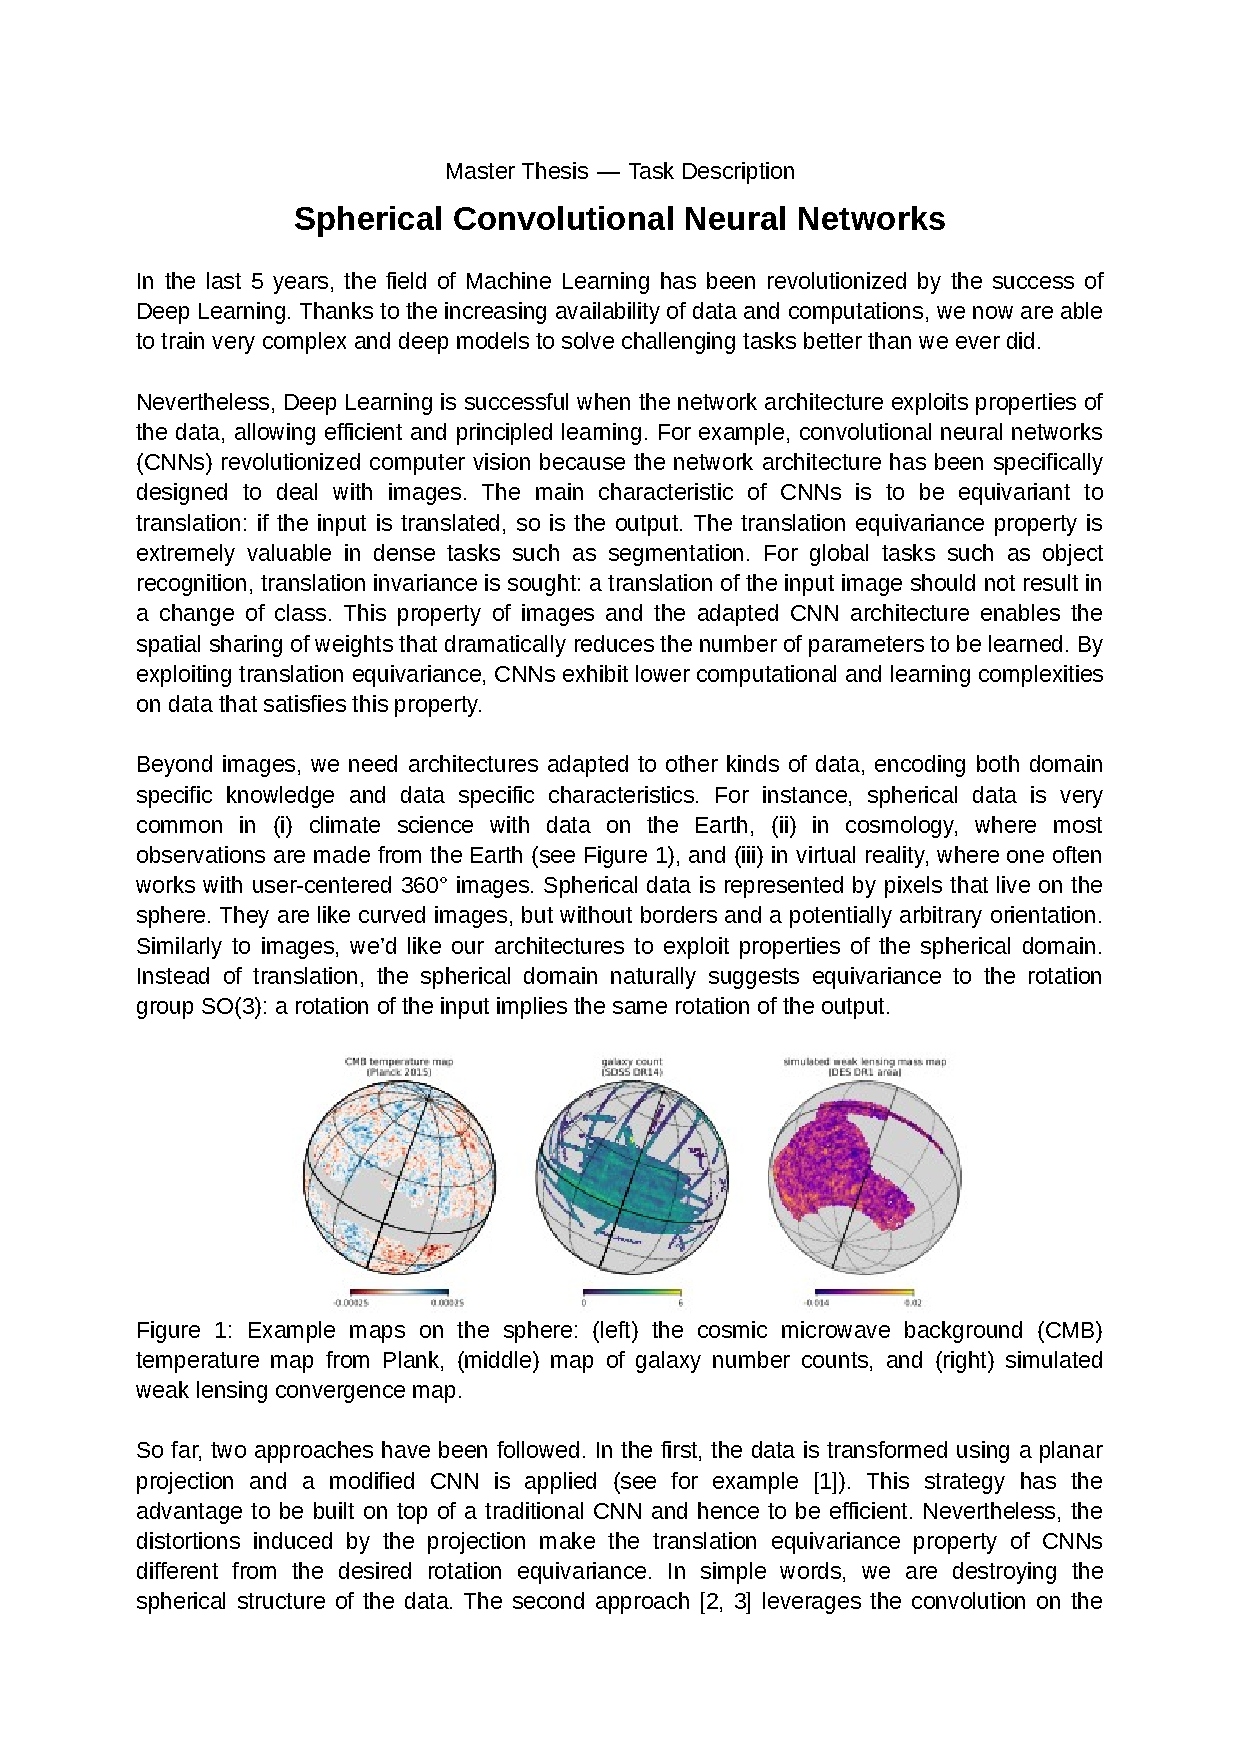
\includepdf[pages=-]{report/master_thesis_proposal_v2.pdf}
% \cleardoublepage
% \thispagestyle{empty}
% \mbox{~}
% \cleardoublepage
\begin{abstract}
%     CNNs are powerful tools in deep learning mainly due to their ability to exploit the translational symmetry present in images, as they are equivariant to translations.\\
% Nowadays, more and more data present different types of symmetries (e.g. rotations), and lie on the sphere $S^2$ (e.g. cosmological maps, omni-directional imaging, 3D models, ...). It is therefore of interest to design architectures that exploit the structure of the data and are equivariant to the rotation group SO(3).
% Different architectures were designed to exploit these symmetries, such as 2D convolutions on planar projections, convolutions on the SO(3) group, or convolutions on graphs. The DeepSphere model approximates the sphere with a graph and performs graph convolutions.\\
% In this study, DeepSphere is evaluated against other spherical CNNs on different tasks to compare their speeds and their performances. The graph convolution is roughly 3 times faster than the SO(3) convolution with the same amount of learnable parameter. It can be up to 10 times faster with less parameters and still give similar results. While the SO(3) convolution is equivariant to all rotations in SO(3), the graph convolution is only equivariant to the rotations in $S^2$ and invariant to the third rotation. Our comparison on SHREC-17 (a 3D object retrieval task) shows that DeepSphere achieves similar results (2 points of difference on F1 score) to spherical CNNs using SO(3) convolution, thus that equivariance to the third rotation is not necessary for this task. Moreover, DeepSphere is more flexible as it can work with any sampling or partial observations of the sphere.

Convolutional neural networks (CNNs) are powerful tools in Deep Learning mainly due to their ability to exploit the translational symmetry present in images, as they are equivariant to translations. Other datasets present different types of symmetries (e.g. rotations), or lie on the sphere $S^2$ (e.g. cosmological maps, omni-directional images, 3D models, ...). It is therefore of interest to design architectures that exploit the structure of the data and are equivariant to the 3D rotation group SO(3). Different architectures were designed to exploit these symmetries, such as 2D convolutions on planar projections, convolutions on the SO(3) group, or convolutions on graphs. The DeepSphere model approximates the sphere with a graph and performs graph convolutions. \\
\indent In this study, DeepSphere is evaluated against other spherical CNNs on different tasks. While the SO(3) convolution is equivariant to all rotations in SO(3), the graph convolution is only equivariant to the rotations in $S^2$ and invariant to the third rotation. Our experiments on SHREC-17 (a 3D shape retrieval task) show that DeepSphere achieves the same performance while being 40 times faster to train than Cohen et al. \cite{cohen_spherical_2018} and 4 times faster than Esteves et al. \cite{esteves_learning_2017}. Equivariance to the third rotation is an unnecessary price to pay. 

In order to prove these results, DeepSphere was tested on the similar dataset ModelNet40 (a shape classification task), and similar results as obtained by Esteves et al. were achieved. The odd behaviour with rotations (the performance worsens in presence of rotation perturbations) may be inherent to the task and the classes, instead of the models or the choice of the sampling scheme.

Finally, regression tasks (both global and dense) were performed on GHCN-daily to prove the flexibility of DeepSphere with a non-hierarchical and irregular sampling of the sphere. The sCNN performed better than simply learning on the time series for each nodes.

Code and experiments are available at \url{https://github.com/Droxef/PDMdeepsphere}.
\end{abstract}
\vfill
\newpage
\thispagestyle{empty}
\mbox{~}
\cleardoublepage
\thispagestyle{empty}
\setcounter{secnumdepth}{3}
\setcounter{tocdepth}{2}
\thispagestyle{empty}
\clearpage
\pagenumbering{gobble}
\tableofcontents
\thispagestyle{empty}
\clearpage                        % New section, with numbering
\pagenumbering{arabic}
\chapter{Introduction}
\setcounter{page}{1}

\section{Motivation}
\paragraph*{}
The field of Machine Learning was changed radically with the apparition of Convolutional Neural Networks \cite{boureau_theoretical_2010}. Their popularity comes from their ability to exploit the translational symmetry present in images. Indeed, the CNN is equivariant to translations due to the weight sharing of the kernel of the filters, meaning that all pixel will go through the same convolution and an element will react identically wherever it is in the image. Then the model does need to learn a single kernel for all the pixels instead of one for each. Furthermore, this invariance does not need to be learned, thus reducing the learning time and increasing the performance.

Symmetries are often present in data, but practically never exploited. Taking the CNN as an inspiration, other symmetries could be exploited, and new deep learning architectures and operations could be designed to be invariant or equivariant to them. 
\section{Problem identification}
\paragraph*{}
In 3D data, and more specifically for spherical signals on $S^2$, the symmetries of interest are rotations. An idea was to leverage the classical CNN to rotational symmetries on spherical signals.

The DeepSphere model \cite{perraudin_deepsphere:_2018} is one of the spherical CNNs created for this purpose. In order to reach an efficient spherical convolution equivariant to rotations and peak performance, hypotheses were made.

The goal of this thesis is to compare DeepSphere against different spherical convolutional neural networks (SCNNs) to see the influence of the hypotheses and differences with the SCNNs, and put forward the advantages of DeepSphere.

\paragraph*{}
First, different tasks, with meaningful datasets, will be analyzed to filter the most interesting ones. These tasks should have sufficient results in other publications of spherical CNNs to have a reference point. Furthermore, these tasks should put forward the differences of DeepSphere with the other SCNNs to be able to show their impact on the performance. 

Then DeepSphere will be adapted to run these tasks and its performance will be compared to existing results.

\section{DeepSphere}
\paragraph*{}
DeepSphere is a graph convolutional network, which works on spherical data and leverages convolutions and hierarchical pooling on graphs, achieving rotation equivariance, computational efficiency and flexibility \cite{perraudin_deepsphere:_2018}.

\clearpage
\begin{figure}[!ht]
    \centering
    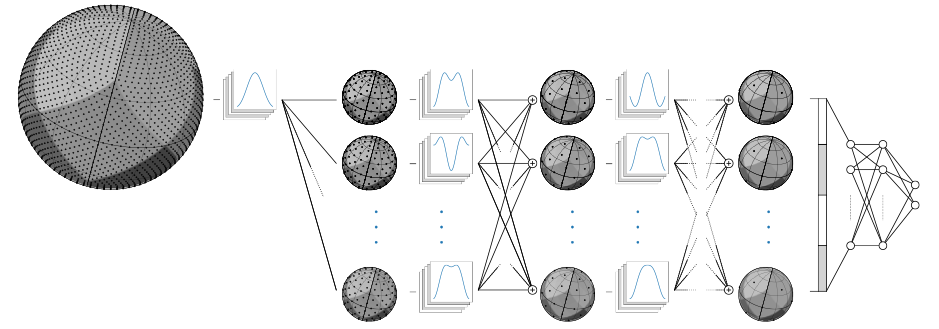
\includegraphics[width=0.8\linewidth]{figure2-Blogpost-SCNN.png}
    \caption{DeepSphere architecture}
    \label{fig:deepsphere}
\end{figure}

\paragraph*{}
A graph is constructed with the idea of data lying on the sphere $S^2$, thus presenting the symmetry of this group. This data consisted originally of cosmological maps, but can be applied to any other data fitting this description.

An important point to precise is that DeepSphere deals with the signal on the sphere, and therefore on the graph. Thus it is not the graph itself that is equivariant to rotations but the operations defined on it, such as the convolution, that are rotation equivariant.

\paragraph*{}
This graph approximating the sphere $S^2$ and using HEALPix \cite{gorski_healpix_2005} sampling scheme initially, has some interesting properties. The eigenvectors of its Laplacian approximate the spherical harmonics. Using these as an orthogonal basis for the graph filter leads to a structure equivariant to rotation. As it only approximates the spherical harmonics, the equivariance to rotation is not perfect either.

The eigenvectors only move towards spherical harmonics with the number of pixels $N~\rightarrow~\infty$ under the conditions studied by \cite{milani_about_nodate}.

% Furthermore,  only correctly equivariant if graph approximates the whole sphere. If the part is too small, the eigenvectors wont approximate the spherical harmonics.

\paragraph*{}
Initially, the graph convolution is performed on the spectral domain using the eigenvectors of the Laplacian \cite{bruna_spectral_2013}. To avoid the heavy computation of the graph Fourier transform, the eigendecomposition of the Laplacian, it is possible to use the Tchebyshev polynomial filter \cite{defferrard_convolutional_2016} for a local filter. Thus, the graph convolution is similar to a classical CNN as the convolution is performed in the spatial plane as a sum of weighted neighbors. The neighbors in the graph are regrouped in hops matching the order of the Tchebyshev polynomial \cite{defferrard_convolutional_2016}.

\paragraph*{}
Using such an isotropic filter leads to equivariance to rotation for $S^2$ group, but the model is invariant to the third rotation of the $SO(3)$ group. Indeed, the filter deals with neighbors in hops around the node of interest, and rotation of the signal around the pixel will not change the response.
Another precision is that the graph approximates the $S^2$ manifold, therefore only two of the $SO(3)$ rotations can be represented on it.



\paragraph*{}
In summary, the key points to take into account are (1) the computational efficiency, (2) the (approximative) rotation equivariance, (3) the flexibility of the model, and (4) the isotropic filters.

\section{Related works}
\subsection{Sphere}
\paragraph*{}
The main reason to use spherical signals is to exploit the rotational symmetry of the sphere $S^2$ or group $SO(3)$. Indeed, some data present symmetry of rotation, thus even after undergoing a rotation transformation, the instance remains fundamentally the same, and its features captures its properties and its state (the orientation of the signal in the space).

\subsubsection{$S^2$ and $SO(3)$}
\paragraph*{}
In this section, there is an explanation of these important notions to clarify them.

$SO(3)$ is the group gathering all the rotations from $R^3$. They correspond to yaw, pitch and roll. This group represents the rotational symmetries of an object, and thus all its potential orientations.
        
The sphere $S^2$ is the 2-dimensional manifold embedded in $R^3$ corresponding to the surface of the ordinary sphere. It is not a group in mathematical terms as there is no composition for points on the sphere. This manifold can be parameterized with only two rotations as it is simply a surface.

\subsubsection{Fourier and Spherical harmonics}
\paragraph*{}
A spherical signal can be represented as a sum of spherical harmonics ($S^2$) or Wigner D-functions ($SO(3)$)\cite{cohen_convolutional_2017}. These functions form an orthogonal basis and are similar to the Fourier mode \cite{driscoll_computing_1994}.
        
\paragraph*{}
The spherical signal has a similar operation to those of time series or euclidean space signals. The spherical harmonics correspond to the frequencies. And in the case of band-limited signals, these spherical harmonics are represented until $l_{max}$ which is the maximum order found in the signal. 

\subsubsection{Discretization}\label{sec:sampling}
\paragraph*{}
In many fields such as computer analysis and Deep Learning, it is not possible to work with continuous signals. Therefore, the signals are discretized to be used correctly. Even if the 2D plane has an optimal uniform discretization, which is the regular grid, there is no such discretization for the sphere $S^2$ \cite{perraudin_deepsphere:_2018}\cite{cohen_spherical_2018}\cite{driscoll_computing_1994}.
There exist different samplings, which can have the following properties:
        \begin{itemize}
        \setlength\itemsep{0.1em}
            \item[-] Iso-latitude: this allows a fast Fourier transform and fast computation of spherical harmonics.
            \item[-] Hierarchical pixelization: useful for pooling operation.
            \item[-] Same-area coverage: each pixel has the same importance as it covers the same area on the sphere.
            \item[-] Uniformity: how well the sampling spans the sphere.
        \end{itemize}
        
Several discretizations are analyzed, and described with their properties hereafter.

\begin{description}
    \item[Equiangular] (also called equirectangular):\\ 
    Equiangular is the most intuitive and widespread discretization of the sphere. It corresponds to a regular grid in the polar coordinate system, the latitude ($\phi$) and longitude ($\theta$), equispaced in the coordinate system, therefore intuitive to understand. A bandwidth L is fixed, corresponding to the maximum frequency (spherical harmonic order) that can faithfully be represented. The grid is composed of 2L latitude rings and up to 2L longitude pixels per ring.
            
    This sampling is iso-latitude and hierarchical, so pooling and SHFT can be done rather easily on them.
    Nowadays, it is widely used for any spherical signal representation such as omnidirectional imaging or cartography. But it has a main downside as the pixels do not have the same area coverage, meaning that some parts of the sphere (the poles) are more densely pixelated, leading to redundant information.
    Additionally, the planar projection of this grid has a lot of deformation in the regions of the poles for the same reasons.
    
    Different sampling schemes based on this idea are presented below:
    \paragraph*{}
    \begin{minipage}{0.7\linewidth}
            \begin{itemize}
            \setlength\itemsep{0.5em}
                \item Driscroll-Healy \cite{driscoll_computing_1994}\\
                It is the oldest and simplest sampling, and thus it is widely used for planar projection, e.g in cartography or omnidirectional imaging.
                One of the pole is represented by 2L pixels because the last ring has a radius of 0, aggravating the redundancy of the sampling. These 2L pixels are, in fact, only a single pixel.
                $$\theta_i = \pi i/2L, \phi_j = \pi j/L$$
                for $i,j = 0, \ldots, 2L-1$
                \item SOFT \cite{healy_ffts_2003}\\
                This version of the equiangular sampling is an upgrade of the previous and was created in order to use a faster theorem for $SO(3)$ Fourier transform.
                Here, the poles are no longer a part of the sampling, but the pixel density is still lower at the equator than near the poles.
                $$\theta_i = \pi (2i+1)/4L, \phi_j = \pi j/L$$
                for $i,j = 0, \ldots, 2L-1$
                \item Gauss-Legendre \cite{keiner_fast_2008}\\
                The difference with this sampling is that it uses the Gauss-Legendre quadrature of the sphere to find the L latitude rings, and the longitude pixels are equiangular spaced. It is used mainly to construct the exact Spherical Harmonics Transform from its samples.
                Apart from that, there is not much difference to the classical equiangular sampling scheme.
                % $$\theta_i = \textrm{Gauss-Legendre nodes}, \phi_j = \pi j/(L+1)$$
                % for $i = 0, \ldots, L, j = 0, \ldots, 2L+1$
                % \item Clenshaw-Curtis \cite{gimbutas_fast_2013}
                % This sampling scheme is built the same way as the previous one but using the Clenshaw-Curtis quadrature.
                % $$\theta_i = \pi i/2L, \phi_j = \pi j/(L+1)$$
                % for $i = 0, \ldots, 2L, j = 0, \ldots, 2L+1$
            \end{itemize}
            \end{minipage}
        \begin{minipage}{0.3\linewidth}
        % \begin{figure}[!ht]
            \centering
            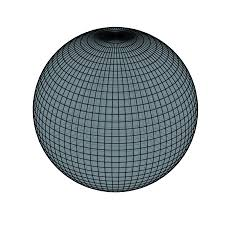
\includegraphics[width=\linewidth]{figures/equi_sphere.jpg}
            \captionof{figure}{Equiangular sampling scheme \cite{perraudin_deepsphere:_2018}}
            \label{fig:equi_sphere}
        % \end{figure}
        \end{minipage}
        % \item[Optimal dimensionality] \cite{khalid_optimal-dimensionality_2014}: \\
        % This sampling scheme focus on reducing the necessary number of pixels to compute an accurate SHT for band-limited signals. It is iso-latitude with L latitude rings, and require $2k+1$ equispaced pixels for each $\phi_k$ ring. One can observe that the number of pixels corresponds to the spherical harmonics up to $l_{max}$, with each ring being a different mode. The reduced number of pixels let achieve a better uniformity, thus the name: Optimal dimensionality.
        %     % $$\theta_i = \pi i/2L, \phi_j = \pi j/L$$
        %     % for $i = 0, \ldots, 2L, j = 0, \ldots, 2L+1$
        %     % and reordered.
        % \begin{figure}[!ht]
        %     \centering
        %     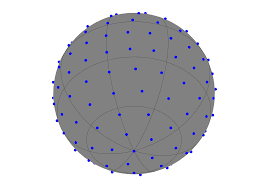
\includegraphics[width=0.3\linewidth]{figures/opt_dim.png}
        %     \caption{Optimal dimensionality sampling scheme \cite{khalid_optimal-dimensionality_2014}}
        %     \label{fig:opt_dim}
        % \end{figure}
        \clearpage
        \item[Geodesic polyhedron] \cite{baumgardner_icosahedral_1985}:\\
        To have the most uniform repartition and equally distributed pixels as possible, different platonic solids can be used: the tetrahedron, the cube, the octahedron, the dodecahedron and the icosahedron. 
        To have a denser sampling, one has to subdivide each face and project the new points on the sphere. Therefore, by construction, this sampling scheme is hierarchical and the pixels have same-area coverage, although some distortion appear for border pixels.
        \begin{figure}[!ht]
            \centering
            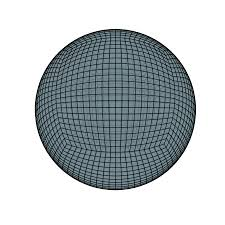
\includegraphics[width=0.3\linewidth]{figures/cube_sphere.jpg}
            \caption{equiangular cubed-sphere grid \cite{ronchi_cubed_1996}}
            \label{fig:cube_sphere}
        \end{figure}
        
            \item[HEALPix] \cite{gorski_healpix_2005}:\\
            ``HEALPix is a Hierarchical, Equal Area, and iso-Latitude Pixelisation of the sphere designed to support efficiently (1) local operations on the pixel set, (2) a hierarchical tree structure for multi-resolution applications, and (3) the global Fast Spherical Harmonic transform'' \footnote{\url{https://healpix.jpl.nasa.gov/html/intro.htm}}
            
            It is based on a rhombic dodecahedron. This sampling scheme is popular especially in cosmology and astrophysics. It presents all interesting features.
            \begin{figure}[h!t]
                \centering
                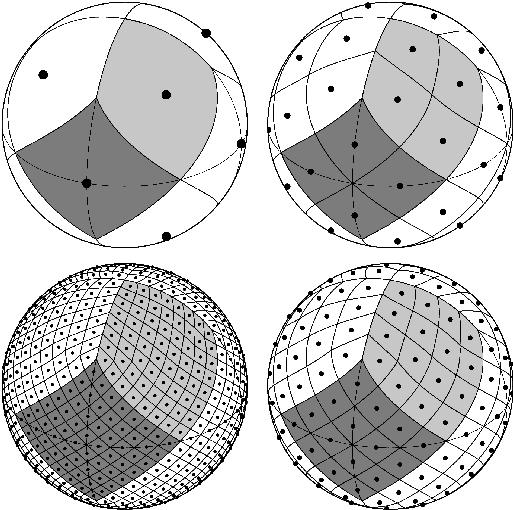
\includegraphics[width=0.3\linewidth]{gorski_f1.jpg}
                \caption{HEALPix tesselation}
                \label{fig:healpix}
            \end{figure}
            % \item[Uniform sampling]:\\
            % No regular, hierarchical, but .
        \end{description}
\paragraph*{}        
There are more sampling schemes that are not presented here. They were not considered for this study, as no spherical CNNs seems to have used any of them. An in-depth analysis of different samplings had been carried out by Elahi et al \cite{elahi_comparative_2016}. The geodesic polyhedron sampling is also to be mentioned of interest as a great number of studies focused on this sampling scheme, but will not be investigated any further on this current report as it is not the goal of the thesis.
In the end, only two sampling schemes will be used on this study: (1) HEALPix due to the variety of its properties and the fact that an interesting graph already exists, and (2) equiangular due to its wide use in most of the fields working with spherical representations (e.g. omnidirectional imaging) in order to demonstrate the flexibility of DeepSphere. An equivariant to rotation graph is planned to be built, specifically for this project.

         
\section{Invariance and equivariance}
\paragraph*{}
An important aspect of this study is invariance and equivariance to transformation, more precisely rotation in the scope of this report. In simple terms, invariance is a property held by a group that is not affected by a specific transformation, as equivariance is a symmetry for functions. So, when affected by a specific transformation before the function, the result is the same as applying another transformation to the output of the function.
More precisely, equivariance exists if the next equation applies.

% \todo{complete}
\begin{equation}
    T_1(f(X)) = f(T_2(X))
    \label{equ:equivariance}
\end{equation}
where:
\begin{itemize}
    \item[$T_i$] a transformation operation (e.g. a rotation)
    \item[$f$] a filter
    \item[$X$] the data analyzed
\end{itemize}
\paragraph*{}
Invariance is when $T_2$ is the identity. Thus the result of the filter will always be the same whatever the transformation is, and the descriptor of the data is still the same.

Same-equivariance is when $T_1 = T_2$, so the transformation of the input is the same as the transformation of the output. It is a special case of equivariance. Thus equivariance leads to descriptors that catch the properties of the data linked to the specific transformation. In the case of DeepSphere, the specific transformation is rotation and the properties will be the orientation of the signal.

\paragraph*{}
To take a specific example in Deep Learning, classification tasks are invariant to transformations by definition. Indeed, the goal is to identify data (e.g. object in image, 3D shape, ...) and compute its output. If the data is intrinsically the same even after a transformation, the output should be the same. This invariance is often achieved by using global average pooling at the end of the network. But it is still desired to have an equivariant network before this last step in order to understand correctly the important features from the data.
        
\paragraph*{}
In the case of a classical CNN, the structure is equivariant to translation by construction, making it a powerful tool for image analysis. Unlike a fully connected network, the power of a CNN comes from weight sharing. Each pixel undergoes an operation using the same learned filter. Thus, the pixels of interest will activate the network the same way wherever they are in the image.
        
For other transformation such as rotation, flip or dilation, data augmentation is used to learn the new invariance. Repeatedly showing the different transformations to the model and teaching it that it is the same data will force the model to learn invariant filters. Thus, the learning is faster using directly an equivariant architecture, as the filters are already equivariant to the desired transformations.

Another possibility to reach equivariance is to use a transformation of the input space to translate the new desired transformation into a useful one - translation in case of a CNN. For example, using a polar projection instead of the 2D grid will translate rotation to translation, even if the result is not easily understandable for the human eyes (the euclidean coordinates ($x$, $y$) change to polar coordinates ($\theta$, $\rho$)). But it is not always possible to use this method. For example, the sphere, which has no perfect planar projection, cannot have a transformation where the translation on the projection does translate correctly to the desired rotations.

\subsection{Spherical CNNs}
\paragraph*{}
Architectures that exploit structure and symmetries present in data are powerful because they do not have to learn them and can directly focus on the main features needed for the task. Thus being invariant or equivariant to some symmetries such as translation or rotation in the data domain can speed up the training time, and make the given model more robust to these perturbations.
    % \subsection{spherical CNNs}
\paragraph*{}
More datasets present rotation symmetries or lie on the sphere $S^2$ (different examples are explained in section \ref{sec:tasks}). In this section, architectures working on this kind of data are presented, along with their approach.
\subsubsection*{2D CNNs on planar projection}\label{sec:2DSCNN}
\paragraph*{}
One of the most instinctive use of CNN on spherical data is to use a planar projection of the sphere $S^2$ and apply a standard CNN. However, as it was seen in sec. \ref{sec:sampling}, there is no perfect uniform sampling of the sphere and thus no projection without deformation. 
% To convince oneself, one can reflect on the quadrature problem proven impossible.
    
Then, it is not possible to translate the desired equivariance to rotation to an equivariance to translation, because deformation is induced on the projection (see Fig. \ref{fig:planar_projection}).
\paragraph*{}
One motivation to use a planar projection of the sphere is to be able to use the highly scalable and powerful standard CNN. The idea is to take advantage of the existing tool, and to transform the input data to faithfully represent it in a suitable format for it.

\paragraph*{}
The first natural approach is to use the classical equirectangular projection and use a standard CNN on the resulting image. But the deformation is large at the poles and the idea of weight sharing does not make sense anymore. Furthermore, the square image with borders does not represent the continuity of the sphere. Thus, different ideas were found to get around this problem.

As a response to the problem of the deformation, a different kernel weight in function of the latitude $\phi$ is used in \cite{su_learning_2017}. Unfortunately, this does not resolve the border problem. Others decided to apply the kernels on tangent planes rather that directly on the equirectangular projection (such as \cite{ferrari_spherenet:_2018}), and represented the distorted kernel on the plane.

All these approaches focus more on the distortion free aspect rather than the equivariance to rotation. However, this kind of architecture is mostly used to analyze omnidirectional images and it is argued that rotation equivariance is not necessary, as the images are always oriented with the gravity. That means that the ground will be at the bottom of the image and ceilings and the sky at the top of the image, as images will then unlikely be upside-down.

%\todo[inline]{more and more to cite\\is image good too?}
\paragraph*{}
Other projections are based on the platonic solids, such as the cubed sphere \cite{boomsma_spherical_2017}, or the icosahedron \cite{lee_spherephd:_2018}. In this case, each face is a planar projection, and instead of using padding, the missing values are taken directly on the adjacent faces.
Using this projection, the equivariance is not guaranteed, and needs a corresponding filter \cite{cohen_gauge_2019}. But depending on the task, this equivariance is not always necessary, as explained in \cite{jiang_spherical_2019}.

Any other sampling scheme presented, and more specifically the polyhedron, can be used for this kind of spherical neural network. There is even a case of a HEALPix projection in \cite{krachmalnicoff_convolutional_2019}.
    
\paragraph*{}
These projections, at best, can only reach perfect discrete rotation equivariance, the rest is only approximation. However, this method still performs well, is scalable and fast, has local filters and operates in the spatial domain.  

    \begin{figure}[h!t]
        \centering
        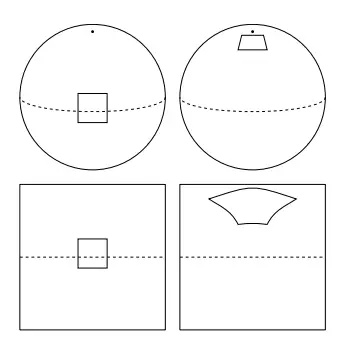
\includegraphics[width=0.5\linewidth]{v2-9d6a9d92bb02bc9e198c4c16397ce2fd_b.jpg}
        \caption{Deformation of planar projection \cite{cohen_spherical_2018}}
        \label{fig:planar_projection}
    \end{figure}

\paragraph*{}
As shown in the work of Cohen \cite{cohen_group_2016, cohen_gauge_2019, cohen_intertwiners_2018}, the difference between isotropic and anisotropic filters is important. Anisotropic filters, also called regular feature fields, are filters that have different weights for each neighbor, opposed to DeepSphere filters, that have a weight for a hop of neighbors, and react the same way wherever an important neighbor is.
They perform generally better than scalar feature fields (isotropic filters) on tasks where the direction is an important feature.

Furthermore, the gauge transformation used by Cohen let him have all kinds of equivariance (from Equ. \ref{equ:equivariance}, $T_2$ can be chosen to fit the needs), which permits flexibility superior to the same-equivariance generally proposed, and seen in DeepSphere.
    
\subsubsection*{Spherical Harmonics Fourier Transform}\label{sec:SHSCNN}
\paragraph*{}
Similar to the case with images, in order to reach true equivariance and find correct convolution, one needs to use Fourier transform and go in the spectral domain. Depending on the group of symmetry one wants to use, the Fourier modes correspond to Spherical Harmonics for the group $S^2$ and to the Wigner D-functions for the group $SO(3)$. 

Theoretically, convolutions in the spectral domain of $SO(3)$ are perfectly equivariant to rotation for continuous signals, using the properties of the symmetry group. 
Using a discretized signal leads to small errors, and is exact only for band limited functions, because the high frequencies (spherical harmonics or Wigner D-functions) are not represented correctly and disappear in the spectral domain.

Models using this method will be called SHFT-CNNs in this report.

\paragraph*{}
Taking into account that the spherical signals lie on the sphere $S^2$, it seems normal to use the spherical harmonics to achieve a convolution equivariant to rotation \cite{esteves_learning_2017}. 
New faster Spherical Fourier transform (SFT) were developed to reach the goal of having this convolution.
% filters defined in spectral domain
% spectral pooling possible

However, the space of moves on the sphere is more complex, and the whole $SO(3)$ group must be considered to be as accurate as possible according to \cite{cohen_spherical_2018}. Different models based on this idea emerged \cite{kondor_clebsch_2018, feng_discriminative_2018}. As well as the $S^2$ counterpart, new SFT for $SO(3)$ were developed to obtain convolutions that are equivariant to rotation.

All these methods use an equirectangular grid to represent the data. This is probably due to SFT being mainly developed for a specific sampling scheme \cite{healy_ffts_2003}. Indeed, the SFT algorithms depend on the chosen sampling and cannot easily be translated to another.
\paragraph*{}
The main problem with this method is that the Fourier transform must be computed for each forward and backward pass during the training of the neural network. This is computationally expensive, even when using a Fast Fourier transform algorithm.

\paragraph*{}
It is possible to expand this methodology to other groups of symmetry, and using translations as well, such as in \cite{weiler_3d_2018} or \cite{worrall_cubenet:_2018}. In this case, the data is not spherical anymore. This goes beyond the scope of this study.
    
\subsubsection*{Graph CNNs}\label{sec:GCNN}
\paragraph*{}
Another way to represent the data that seems more and more used, is to use a graph to approximate the manifold where the data lies. It is then possible to use a graph-CNN on this representation (e.g. in \cite{bruna_spectral_2013} or \cite{masci_geodesic_2015}). The graph convolution is designed in the Fourier domain as there is no meaningful translation operator in the vertex domain \cite{defferrard_convolutional_2016}. Thus it is the same as applying a graph filter, using the Laplacian eigenvectors, with the main downside being the expensive graph Fourier transform, to perform each time. Indeed, there is no FFT generalized for graph Fourier Transform.
\paragraph*{}
The advantage of graphs is that they can use any coordinates and sampling, thus fitting any data and going beyond classical euclidean domain. This is the case for MoNet \cite{monti_geometric_2016}, which regroups different Graph Convolutional Neural Networks and devised a more general framework from the others, learning the weight function, which is fixed in other representations. A review on Deep Learning on graph can be found in \cite{bronstein_geometric_2017}.

\paragraph*{}
To fit the spherical data, a graph approximating the sphere $S^2$ is a logical choice, since this same choice is made for cosmological map classification with DeepSphere \cite{perraudin_deepsphere:_2018} and omnidirectional images representation \cite{khasanova_geometry_nodate, frossard_graph-based_2017}.
Furthermore, to have more computationally efficient graph convolution, the expensive eigendecomposition can be avoided by replacing the filters with a polynomial function of the Laplacian \cite{defferrard_convolutional_2016, frossard_graph-based_2017}. However, this applies only for localized filters. The order of the polynomial function $K$ can be seen as the number of neighboring hops a localized kernel can interact with.

At the same time, as the kernel sees rings of neighbors, the hops from the localized pixel, it has no idea of orientation, resulting in an isotropic filter. Thus, some information may be lost, and in terms of image processing, these filters can only detect blobs of pixels, not edges or directional changes of intensity\footnote{\url{https://twitter.com/TacoCohen/status/1123736021546545156}}.
    
\paragraph*{}
All these spherical CNNs are task-agnostic and can be adapted for any task, as long as the input can be explained in terms of a graph (e.g. a spherical signal for DeepSphere). 
Nonetheless, it can be domain specific if the model is dependant of a specific coordinate system.


\chapter{Methodology}\label{chap:Datasets}
\paragraph*{}
As the goal of this study is to compare DeepSphere \cite{perraudin_deepsphere:_2018} against several other spherical CNNs to show its advantages and the impact of the differences with the SCNNs and the hypothesis made, the first step to do is to find different tasks to work on and the datasets linked to them. 
These tasks must have results from different spherical CNNs in order to compare them with DeepSphere results, and challenge the different aspects of DeepSphere. Another set of tasks has to be chosen such that it puts forward DeepSphere's advantages, where few of the other models could compete on these properties.

\paragraph*{}
As a reminder, the main advantages of DeepSphere are: 
\begin{itemize}
\setlength\itemsep{0.07em}
    \item[-] The convolution is similar to a traditional CNN: A weighted sum of neighbors, leading to a fast computation.
    \item[-] Flexibility: Any sampling can be used, as long as a graph can be built, even if the sampling covers only part of the sphere, or the sampling is irregular.
\end{itemize}


More importantly, the differences and hypothesis made that have a yet unkown influence:
\begin{itemize}
\setlength\itemsep{0.07em}
    \item[-] By construction, the convolution is only equivariant to rotation on $S^2$ (the graph approximates this manifold). The convolution is invariant to the 3\textsuperscript{rd} rotation presents only in $SO(3)$.
    \item[-] The filters are isotropic.
    \item[-] The equivariance to rotation is theoretically not perfect, due to graph construction.
\end{itemize}


% \section{Implementation}
% \todo[inline]{What to put in here}
% \todo[inline]{methodology speak about deepsphere, main points, refer to paper rather than to say all again}


\section{Different tasks} \label{sec:tasks}
\paragraph*{}
This study focuses only on supervised task, and a list of potential interesting ones is presented below.
% \begin{itemize}
%     \item global classification
%     \begin{itemize}
%         \item classification
%         \item shape retrieval
%     \end{itemize}
%     \item global regression
%     \item dense classification
%     \begin{itemize}
%         \item object detection
%         \item segmentation
%     \end{itemize}
%     \item dense regression
% \end{itemize}
\begin{itemize}
    \item Cosmological models classification
    
    This is the original task from \cite{perraudin_deepsphere:_2018}.
    The goal of this task is to discriminate cosmological maps simulated with two different sets of parameters.
    The main problem with this task is the high-density of the data, and the fact that the necessary features to discriminate the models are small and will be lost if the maps are down-sampled too much. Thus SHFT-SCNNs (cf. section \ref{sec:SHSCNN}) cannot be trained in a reasonable time.
    \item Proof of concept classification or segmentation
    
    For a majority of SCNNs, mock datasets are standard 2D images that are projected on the sphere. They are called mock datasets because they are 2D images and are artificially transformed to a spherical signal. Unfortunately, this is often senseless, as no real signal could be similar to them. Therefore, it does not make sense to use this type of tasks to compare DeepSphere with the others as they are designed to prove the good functioning of the spherical models.
    
    The most popular example of this type of task is the projected MNIST dataset, used by a great number of publications such as \cite{cohen_spherical_2018, cohen_gauge_2019, khasanova_geometry_nodate, frossard_graph-based_2017, lenssen_group_2018, krachmalnicoff_convolutional_2019, ferrari_spherenet:_2018}. This tasks make the least sense as there is no character recognition on the sphere in real life.
    
    Other mock datasets are PASCAL VOC \cite{su_learning_2017}, a dataset of planar images for object class recognition, or FlyingCars \cite{ferrari_spherenet:_2018}, equirectangular projection of panoramic images with additional 3D model of cars to find. 
    \item Shape retrieval
    
    This task consists in finding descriptors of 3D CAD models in such a way similar models could be retrieved from a single one, minimizing the distance between the descriptors. It is used by \cite{cohen_spherical_2018, esteves_learning_2017, esteves_equivariant_2019}, and the main interest is the fact that the models remain fundamentally the same, even rotated, thus presenting $SO(3)$ symmetry.
    
    ShapeNet and ModelNet are two datasets of CAD models used for this task. 
    \item Shape classification
    
    This task is similar to the previous one, and uses the same datasets, but the goal is only to classify the models, which seems easier. Results for this task are in \cite{esteves_learning_2017, esteves_equivariant_2019, jiang_spherical_2019}.
    \item Scene identification
    
    This task consists in classifying scenes where the configuration is inside-out, the point of view is on the center of the sphere, and the scene viewed is projected onto the outer sphere. The data has the form of panoramas images (equirectangular projections) or point clouds.
    
    Some datasets present in literature are Matterport3D \cite{noauthor_matterport3d:_nodate} used by \cite{esteves_equivariant_2019} or SUN360 used by \cite{lee_spherephd:_2018}.
    
    \item Omnidirectional segmentation
    
    The previous task can be transformed easily into a segmentation problem, to identify the objects within the scenes. The data often consist of omnidirectional images with RGBD channels, and are presented as equirectangular projection or point clouds.
    
    Datasets present in the literature are 2D3DS \cite{armeni_joint_nodate} used by \cite{jiang_spherical_2019, cohen_gauge_2019} or SYNTHIA used by \cite{lee_spherephd:_2018}.
    
    Even if omnidirectional images lie on the sphere, due to the optical properties of the lens, or the type sensor used to capture the images, they do not necessarily present rotation symmetry. Indeed, they are always oriented by gravity (with the ground at the bottom of the image).
    
    \item Climate pattern segmentation
    
    Planetarian data seems a logical approach, as they lie directly on the sphere - the Earth. Planetarian data are all signals evolving on the Earth such as weather, economics or demography.
    Again they do not necessarily present rotation symmetry, as the globe has a single axis of rotation, and the behaviour of the data is not the same on certain parts of the sphere.
    
    A simple signal is the weather, and a task born from this data is the classification of climate or the detection of extreme weather pattern from multiple weather signals. This task is performed by \cite{jiang_spherical_2019, cohen_gauge_2019}.
    
    
    % \item Variable regression on planetary data
    % \item Biology molecular
    
    % \item sphere/part classification
    % \item sphere/part segmentation
\end{itemize}

\paragraph*{}
Of course, many other different tasks that may be pertinent, but those presented were the most represented in the analyzed literature. Another point would be to create our own task from scratch, and it would still be possible to compare the DeepSphere results with the other public spherical CNN ones. But a task, or data, where DeepSphere could be put forward was not found.
% \section{Different datasets}
% \subsection{3D objects}
% Equivariance in rotation useful because the object is the same whatever the orientation is ( an upside down plane is still a plane).

% Main problem is that the spherical signal does not represent correctly the 3D object. occlusions are not represented, and only a specific point of view for each vertex is represented.

% meilleur representation est graph a partir de vertex. Normalement toujours rotation equivariant, même si approxime plus les harmoniques spheriques.

% classifiy only graphs and not signal on graph.

% \subsection{cosmological maps}
% see deepsphere paper

% need a great resolution to observe features
% anisotropic filters is not needed in this case

% \subsection{Omnidirectional imaging}
% real life or virtual.
% True representation on the sphere (depending on the sensor)

% direction of gravity is important
% No real rotation symmetry of signal
% \subsection{panorama}
% Better representation might be the cylinder. In this case, we keep a rotation and the gravity. A plus side is the perfect uniform sampling on the cylinder.
% \subsection{planetarian data}
% pseudo spherical data, easily represented by a graph.
% But there is no rotation symmetry, or only 1 rotation (spin of the earth)

% no similar signal on pole or equator, or on oceans and continents.

% but local rotation equivariance may be useful

% climate

% density, economics,...

% % \subsection{molecular}

% % \subsection{medical imaging}

% \subsection{mocks dataset}
% Mainly projection of plane images on the sphere. For example, projection of MNIST digits.

% do not represent reality, or real life problem. It is not useful at the end. Only to prove some trivial concepts.

\chapter{Benchmark}
\section{Choice of tasks}
%\paragraph*{}
%As the goal of this study is to compare DeepSphere against several spherical CNNs, and prove its advantages, one must chose carefully the tasks. 
% As a reminder the advantages of Deepshere are its speed and its flexibility. Downsides are only equivariant in $S^2$ by construction and invariant to the third rotation in $SO(3)$, and the almost equivariance due to graph construction.
% Thus, the tasks must put forward these differences, and if there is a profit having them.
\paragraph*{}
First, a global task in common with the other sCNNs is chosen, in order to see how well DeepSphere performs against them despite having an invariance to the 3rd rotation. The SHREC17 competition\footnote{\protect\url{https://shapenet.cs.stanford.edu/shrec17/}}, using a shape retrieval task, is selected for this purpose. Cohen \cite{cohen_spherical_2018} and Esteves \cite{esteves_learning_2017} used this task to demonstrate their model efficiency. Their methodology can be reused as well as their results. Another similar dataset with a classification task is chosen as well:  modelNet40\footnote{\url{http://modelnet.cs.princeton.edu/}}. The methodology is similar, and the task is used by Jiang \cite{jiang_spherical_2019}. These two tasks will demonstrate how well DeepSphere performs in comparison to other state of the art spherical CNNs in terms of speed and performance, as well as confirm the influence of the isotropic filter and the imprecision of the rotation equivariance.
\paragraph*{}
The main other aspect that remains to be shown is the flexibility of DeepSphere. To demonstrate this, another sampling can be chosen, using only a part of the sphere, or any spherical signal that is sampled non uniformly over the sphere. Measures on the Earth such as weather, demography or economics is a great example because the Earth can be approximated by a sphere, and the density of measurements is greater on the continents than on the oceans. For this reason, the GHCN-daily \cite{noauthor_global_nodate} dataset is chosen, even if there is no underlying task and no comparison with the other spherical CNNs, as they cannot work with other sampling. 
% In order to work with a new task, a dense regression can be chosen.
\paragraph*{}
Finally, a segmentation task is chosen to demonstrate that DeepSphere can be adapted for any task. A climate event detection task with the Extreme Weather dataset \cite{racah_extremeweather:_2017} or the climate pattern segmentation task \cite{mudigonda_segmenting_nodate} can be chosen. The second one has the advantage to be performed by Jiang \cite{jiang_spherical_2019} and Cohen \cite{cohen_gauge_2019} as well. It is also more interesting as publicated results are available. Both these tasks are on hold due to a lack of time for the experimentations.
\paragraph*{}
All the experiments code is available on Github\footnote{\url{https://github.com/Droxef/PDMdeepsphere}} and they were run on NVIDIA GeForce GTX 1080 Ti GPU with 11GB of memory.

\subsection{Shape retrieval - SHREC17}\label{sec:shrec17}
\paragraph*{}
SHREC17 is the SHape REtrieval Contest of 2017. The goal of this contest is to develop a tool to manage and analyze 3D shapes, in the form of CAD models. The contest focuses more on the retrieval part than classification. Retrieval means to quantify how much a model is similar to another one. In other words the goal is to find good descriptors for these shapes, the retrieved models being the ones with a high similarity/a low distance between descriptors.
More information can be found on their website \cite{noauthor_shrec_nodate}.
\paragraph*{}
The dataset has 51'300 models, unevenly distributed in 55 classes and is a subset of the ShapeNet dataset. The subcategories will not be used for our study as Cohen and Esteves did not use them. It is separated in three sets: training (70\%), validation (10\%) and test (20\%). The class distribution is similar between the sets. Two versions of this dataset exists: an aligned version where all the models have the same natural orientation, and a perturbed version where the models are randomly rotated.
The second one is used by Cohen to test the rotation equivariant representation \cite{cohen_spherical_2018}, and is also chosen in this work for the same reason.
\paragraph*{}
Another advantage of this dataset is that it can be used as a classification task for another comparison as well. Further it seems that there is still room for improvement considering the results of the spherical CNNs and the winners of the contest, which are task-specific models.

\begin{figure}[!ht]
    \centering
    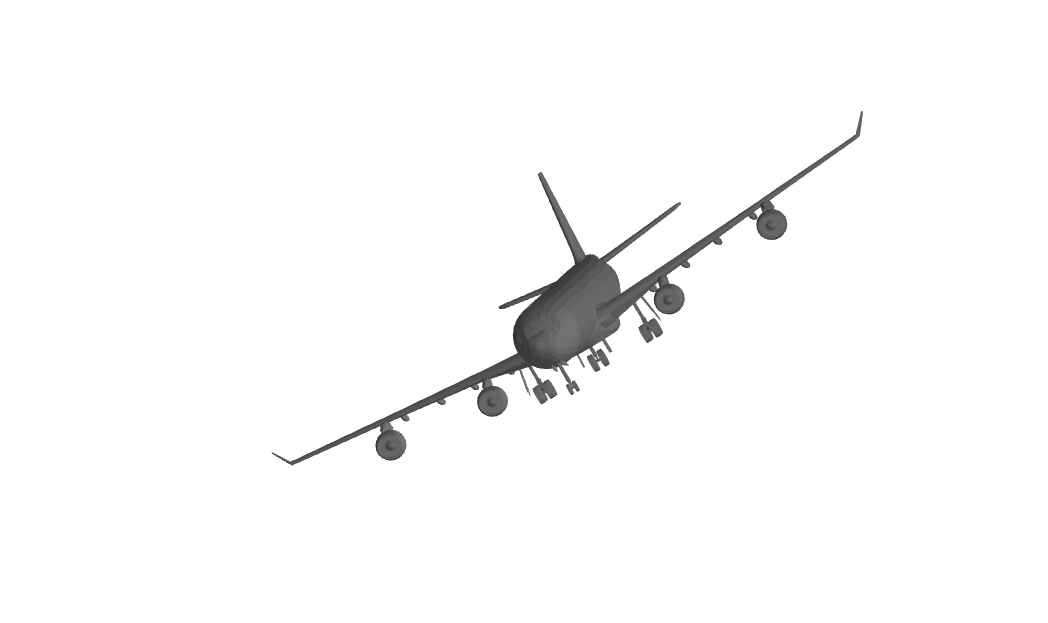
\includegraphics[width=0.6\linewidth, angle=-30, trim={2cm 3cm 2cm 1cm}, clip]{3_front.png}
    \caption{Example of a shape from SHREC17 dataset}
    \label{fig:airplane_shrec17}
\end{figure}

\subsection{Shape classification - ModelNet40}\label{sec:mn40}
\paragraph*{}
The task is global classification of 3D shapes and the data is similar to the previous task as it is a collection of 3D CAD models \cite{zhirong_wu_3d_2015}.
The dataset is a collection of 12'311 models unevenly distributed in 40 classes. It is split in two parts, 80\% for training and 20\% for test. The class distribution is similar between the parts.
Even though a new clean dataset exists with aligned models, the older version was chosen for the same reasons as for SHREC17 (cf. section \ref{sec:shrec17}).

\paragraph*{}
The main advantage to choose a similar task is to reuse the preprocessing and the methodology, and to be able to compare with more available results. The challenge with this specific task is the relatively small size of the dataset, and the fact that some of the classes are not easily distinguishable. For example, it is easy to distinguish an airplane from a stair, but not a flower pot from a vase or a plant.
% airplane\_0119 cannot support a rotation?

% poor population
\subsection{Dense regression - GHCN-daily}
\paragraph*{}
As said earlier, GHCN-daily is a dataset gathering different measurements from over 100'000 weather stations around the globe, with daily measures since 1891 \cite{noauthor_global_nodate}. The main features are meteorological measurements such as temperature, precipitation and snow fall and are represented daily, as suggested by the name of the dataset. More measurements exist, but they are not represented enough to be used correctly.

\paragraph*{}
The main interest for choosing this dataset is that the data lies naturally on a sphere, the Earth, and the pixels, the weather stations, form a non-regular and non-uniform sampling. Indeed, there is a higher concentration in some countries such as USA, Germany or Australia, and almost nothing over the ocean.

\paragraph*{}
There are no specific tasks defined for this dataset, and no spherical CNN or state-of-the-art architecture has been used on it at the time of this study.
The only application found is the  \href{http://jessicastringham.net/2018/06/11/climate-classification-with-neural-nets.html}{climate classification by Jessica Stringham}\footnote{\url{http://jessicastringham.net/2018/06/11/climate-classification-with-neural-nets.html}}.
The first thing to do is to define a task that makes sense. One type of tasks not performed yet with DeepSphere is regression problem, and as features with potential correlation is available, exploring regression is interesting.

\begin{figure}[!ht]
    \centering
    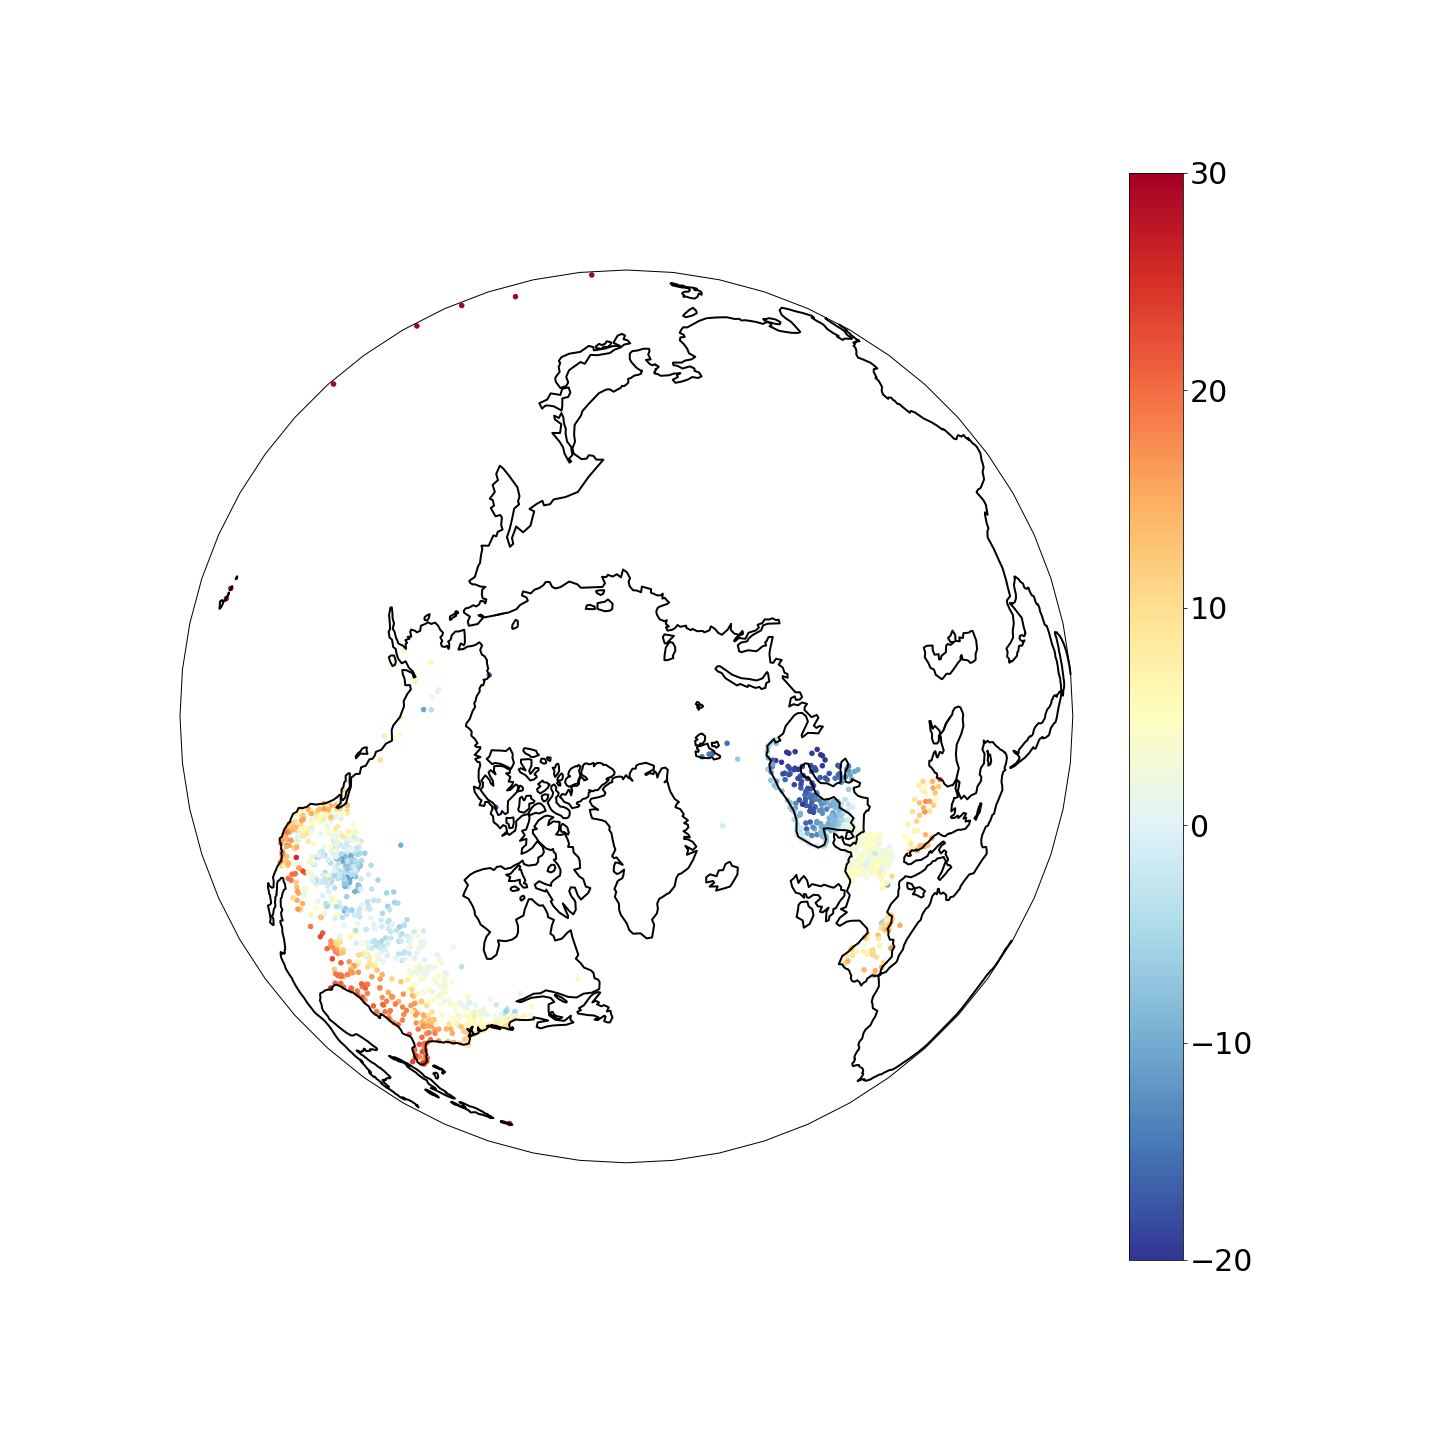
\includegraphics[width=0.6\linewidth]{temp_min.png}
    \caption{Minimal temperature over the Earth}
    \label{fig:temp_min}
\end{figure}
\clearpage
\subsection{Climate event detection - ExtremeWeather}
\paragraph*{}
The ExtremeWeather dataset \cite{racah_extremeweather:_2017} is used for extreme weather events detection based on simulations. It was constructed for the use of CNN, for semi-supervised learning and provides only bounding boxes instead of groundtruth labels for the events.


\paragraph*{}
The data com from CAM5 \cite{neale_description_nodate} that is a meteorological atmospheric model. It is presented on a equiangular projection with a 25-km resolution at equator (a grid of resolution 0.23\degree for longitude by 0.31\degree for latitude), and the different extreme weather events are shown with bounding boxes.

\paragraph*{}
One possible idea is to create a supervised segmentation task, creating labels the same way as in Mudigonda work \cite{mudigonda_segmenting_nodate}. Once the groundtruth labels are found within the bounding boxes, it becomes a dense classification task.

\begin{figure}[!ht]
    \centering
    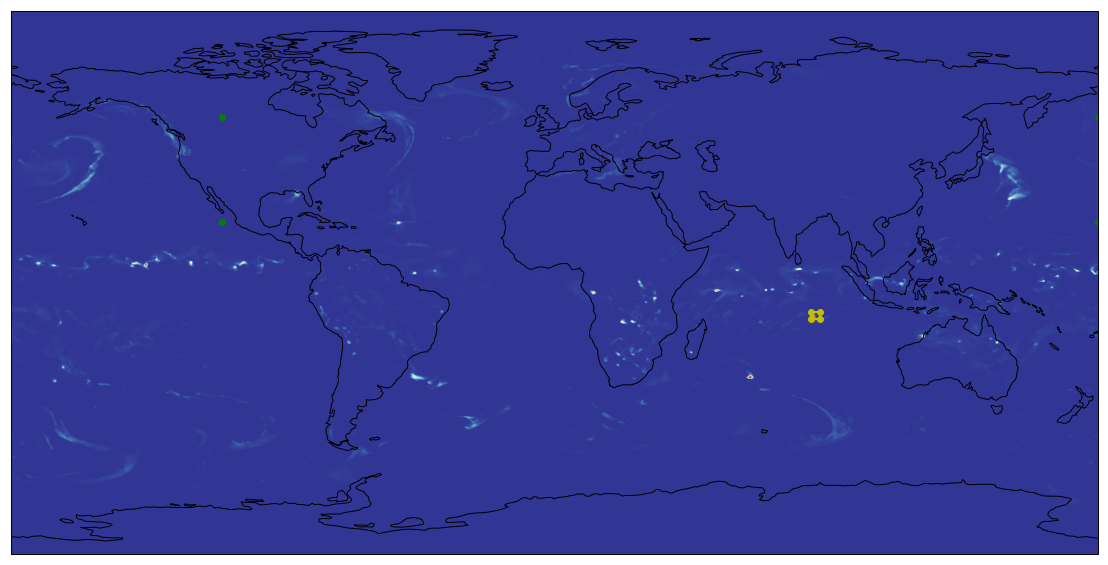
\includegraphics[width=0.99\linewidth]{EW_day1.png}
    \caption{Equiangular projection of precipitation over the earth. Low values are blue and high values red.}
    \label{fig:EW_PREC}
\end{figure}

\subsection{Climate pattern segmentation}
\paragraph*{}
This section is still incomplete as there is not enough time to preprocess the data and do the experiments. But the goal is to perform the same climate pattern segmentation as Jiang and Cohen did, based on the first experiment of Mudigonda \cite{mudigonda_segmenting_nodate,jiang_spherical_2019,cohen_gauge_2019} with a dataset based on CAM5.
% \subsection{just another non uniform dataset}
% Incomplete section, in future works


\section{Previous work}\label{task:cosmo}
\subsection{Cosmological maps classification}
\paragraph*{}
The first problem where DeepSphere was demonstrated is a discrimination problem. The goal was to classify cosmological convergence maps in two models \cite{perraudin_deepsphere:_2018}.
% Further description of the experiment is detailed in the publication.

\paragraph*{}
The maps used the standard cosmological sampling, HEALPix, with a density of\linebreak $N_{side}=1024$, corresponding to $12.5\times 10^6$ pixels per map. As the distribution of the data in the maps is isotropic and homogeneous, the maps were split from 12 parts of sphere to 192 parts of sphere to increase the difficulty of the problem.


\subsection{Comparison}
\paragraph*{}
It is difficult to compare with other spherical CNNs because there are too many pixels and the computation time is too high for Fourier transform, and others were demonstrated with much lower resolution (only $10\times 10^3$ pixels).

It is not possible to reduce the density of the maps too much (less than $N_{side}=512$) as too much information would be lost, and the task would become impossible.

An analysis of the inference time\footnote{It is the time needed to compute a single pass of training for one instance} is computed to show that SHFT-SCNNs cannot compute in a reasonable time the cosmological tasks. The results are seen in Fig. \ref{fig:cosmo_time}, and the missing values are due to (1) not enough memory on the GPU for Cohen's model and (2) to the naive method for computing spherical harmonics for Esteves' model taking too much time (>24h) for $bw=220$. The time for computing the spherical harmonics in the case of Esteves' model is not taken in consideration in this analysis because it is done offline.

\begin{figure}[!ht]
    \centering
    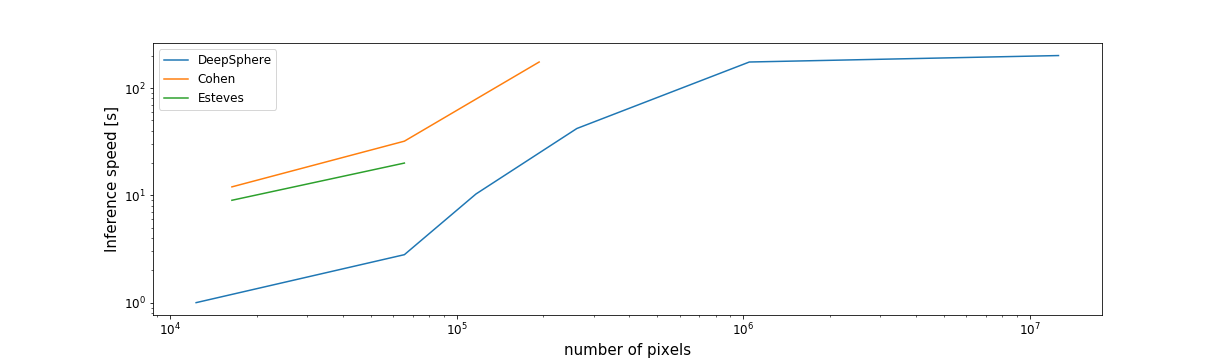
\includegraphics[width=\linewidth]{figures/cosmo_time.png}
    \caption{Analysis of the inference speed for different models and different map density on the cosmological maps classification task}
    \label{fig:cosmo_time}
\end{figure}
% (48th part 0.65s batch 16, 2.9 batch 64)
% 12th part 2.8 batch 16
% 0.165
% 768 parts  0.045 batch 16

% \begin{table}[!ht]
%     \centering
%     \begin{tabular}{c|cc}
%         Models & \# pixels & inference speed \\ \hline
%         DeepSphere order 8 & $16.4\times 10^3$ & 2.8ms \\
%         DeepSphere order 4 & $65.5\times 10^3$ & 10.3ms\\
%         DeepSphere order 2 & $262.1\times 10^3$ & 42ms\\
%         DeepSphere order 1 & $1.0\times 10^6$ & 175ms\\
%         DeepSphere order 0 & $12.6\times 10^6$ & 201ms\\
%         Cohen~\cite{cohen_spherical_2018} ($bw=220$) & $193.6\times 10^3$ & 710ms\\
%         Cohen~\cite{cohen_spherical_2018} ($bw=1773$) & $12.6\times 10^6$ \\
%         Esteves~\cite{esteves_learning_2017} ($bw=220$)& $193.6\times 10^3$ & did not compute SH  \\
%     \end{tabular}
%     \caption{Analysis of the inference speed (time to process a single pass of the model) for different models and different maps on the cosmological maps classification task}
%     \label{tab:cosmo_time}
% \end{table}


\section{Shape retrieval task - SHREC17}\label{task:shrec17}
\subsection{Task presentation}
\paragraph*{}
First, the approach of the other SCNNs are described in order to run the experiments in similar conditions.
Indeed, in order to compare the SCNNs, the same basis much first be achieved.
\subsection{Other spherical models}
\subsubsection{Cohen Model}
\paragraph*{}
Cohen used an equiangular grid following a SOFT sampling scheme~\cite{healy_ffts_2003} to project the data. The original model~\cite{cohen_spherical_2018} uses a bandwidth $bw$ of 128. For the comparison, we will use the version with $bw = 64$ required for the simple model provided in github\footnote{\url{https://github.com/jonas-koehler/s2cnn/tree/master/examples/shrec17}}.

The treatment used by Cohen with its s2cnn is a ray cast of all the pixels from the chosen sampling point in the direction of the center of the sphere. The mesh object is scaled to fit within the unit sphere, the center of mass of the shape being in the center of the sphere. Six features were computed from the rays: distance from the sampling point to the first intersection of the ray and the mesh object, $\cos$ (scalar product) and $\sin$ (cross product norm) between the ray and the normal of the mesh and the 3 same features using the convex hull of the mesh.
\paragraph*{}
The model architecture can be summed up by:
$$\textrm{Cohen}(X) = FC \circ I_{SO3}\circ L_2 \circ L_1$$
where:\\ 
$L_1 = P_{16} \circ ReLU \circ BN \circ F_{S^2/100}$\\
$L_2 = P_{10} \circ ReLU \circ BN \circ F_{SO3/100}$\\
$FC$ is a fully connected layer, $I_{SO3}$ is an integration over $SO(3)$ layer, $P_x$ is a pooling layer to a map with bandwidth $x$, $BN$ is a batch normalization layer and $F_{X/Y}$ is a convolution layer over the domain $X$, where $Y$ is the output features.

\paragraph*{}
Thus, the first layer is always a convolution in $S^2$, as the spherical signal lies on the sphere. The further layers will always be convolutions over $SO(3)$ and the kernel used for the filter has non-local support.

\paragraph*{}
A simpler model gives similar results, has one layer less than the original, uses data with a smaller bandwidth (64 instead of 128) and uses other data augmentation, like random rotations. Finally, the global max pooling from the initial model is replaced by an integration over $SO(3)$ in the simple model. It is observed that the resulting training time is smaller, as the number of parameters is reduced by $10^6$.

\paragraph*{}
We observe that random rotations are added as augmentation in the simpler model, despite being redundant as the structure is rotation equivariant. It may be because the sampling density is different at the poles and the equator, and high frequency information is better represented in high density zones.

\subsubsection{Esteves Model}
\paragraph*{}
The model architecture of Esteves' model \cite{esteves_learning_2017} is much more complex as it is deeper and narrower. Additionally, each feature is treated separately in a different branch, and the results are concatenated before the global average pooling. This original architecture leads to a more robust model.

Batch normalization is also used after each convolution, and a fully connected layer is added after the global average pooling. Additionally, random rotations are used for augmentation, likely for the same reasons as in Cohen's work. The much deeper model allows for a fast learning, and it needs only few epochs to reach peak performance.%, even if this is specific to the task.

\paragraph*{}
The main original elements are:
\begin{itemize}
\setlength\itemsep{0.07em}
    \item[-] the pooling in spectral space, as it is easier to use, acts like a low-pass filter, and an inverse SFT is not needed;
    \item[-] the convolution is in the spherical harmonics domain, and thus is only equivariant to the symmetries of $S^2$;
    \item[-] the use of a localized filter where the spectral space is discretized with a few anchor points and linear interpolation is used;
    \item[-] the global average pooling is weighted by the area of the pixel to take into account the deformation of the equirectangular projection.
\end{itemize}

\paragraph*{}
The same projection and bandwidth as in Cohen's work is used, but only the two first features are kept (the distance to the model and the $\sin$ with the face normal).
\subsection{Implementation}
\paragraph*{}
The data is first preprocessed in order to get a spherical signal. The same preprocessing is used for all models to have the same basis for the comparison.

The principle of the ray casting used by Cohen is sketched in Fig. \ref{fig:ray_cast}. As Cohen did, six features are computed: distance of the ray to the first intersection, $\cos$/$\sin$ with the normal of the mesh and the 3 same features using the convex hull. The resulting spherical signal of the first feature for the same object as the last figure is the Fig. \ref{fig:sphere_signal}.
\begin{figure}[ht]
    \centering
    \includesvg[width=0.5\linewidth]{lamp_000018.svg}
    \caption{Sketch of the ray-casting on a sphere}
    \label{fig:ray_cast}
\end{figure}
\paragraph*{}
The goal to use a spherical signal to represent a complex shape is to take advantage of the symmetries of the sphere. Indeed, 3D shapes have different possible orientations that spans entirely $SO(3)$. Whichever its orientation is, the internal representation of the shape is the same and should be recognized as the same object.

In a general way, the rotational symmetries of any task can be exploited by projecting the data on the sphere $S^2$.

\begin{figure}[ht]
    \centering
    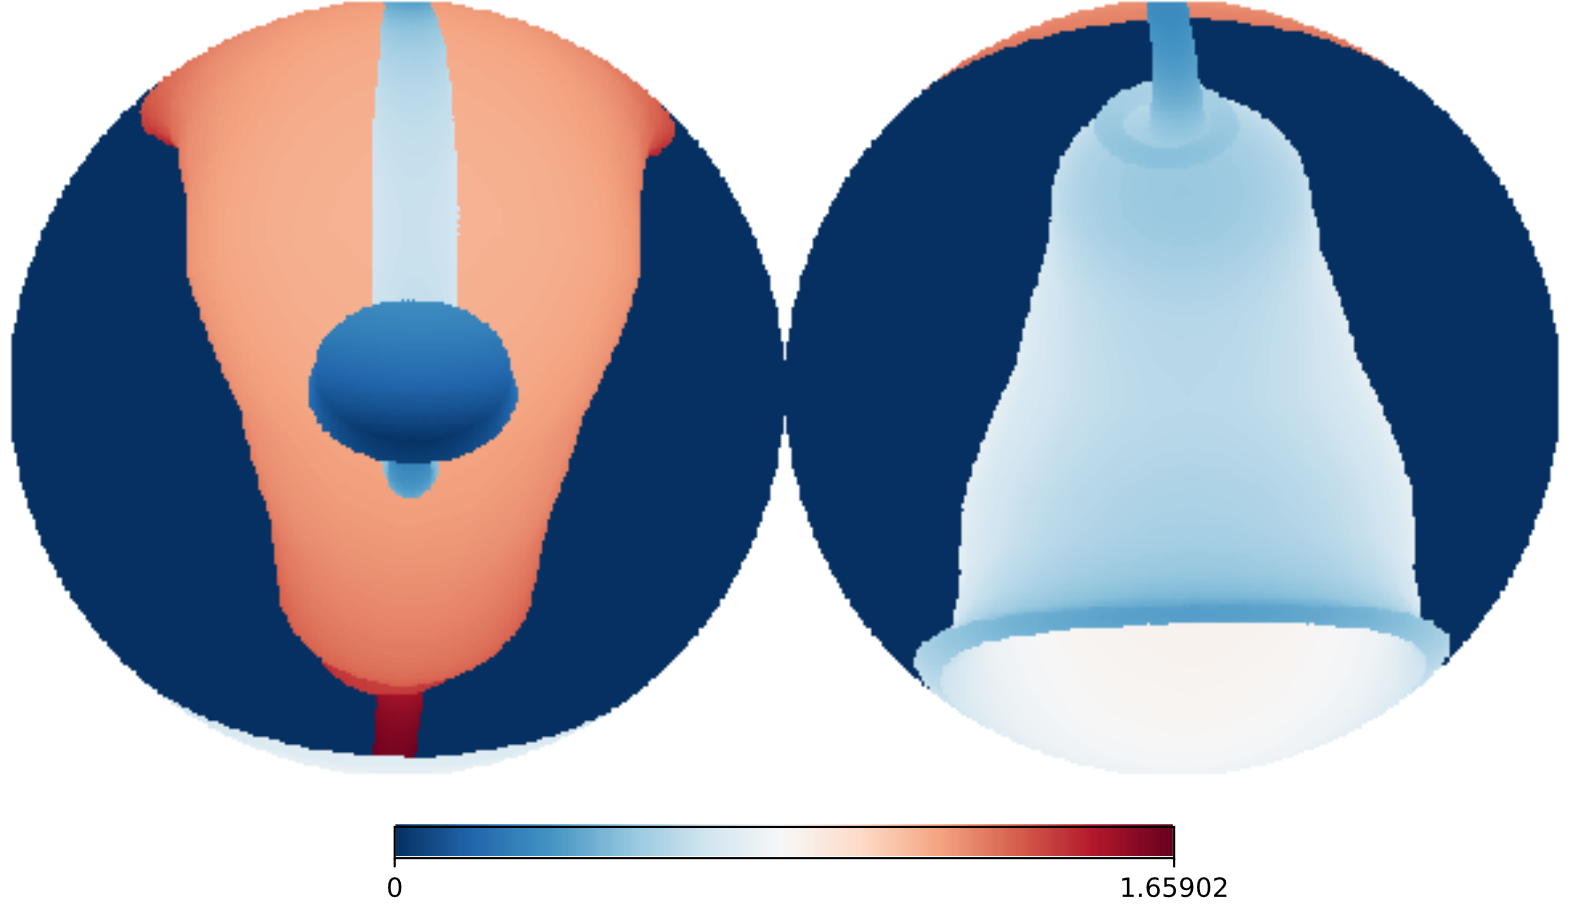
\includegraphics[width=0.5\linewidth]{lamp_sphere_000018.PNG}
    \caption{Back view (left) and front view (right) of the spherical signal obtained by ray-casting the distance from the ray to the first intersection on a sphere.}
    \label{fig:sphere_signal}
\end{figure}
\paragraph*{}
A sampling density compatible with the two comparison models is choosen first. Both models use an equiangular sampling with a bandwidth of 64 resulting in a total number of pixels of $(2*bw)^2\approx16k$. The chosen sampling is HEALPix with an $N_{side}$ of 32, in order to have a similar, but slightly lower, number of pixels.

The data was then normalized to have a normal distribution of mean 0 and standard deviation 1.

\paragraph*{}
As a first step, a similar architecture as in Cohen's simple model is used, which is different than the one Cohen used in his publication. It is assured that the results are similar, and it was rerun to confirm it. 

The DeepSphere model based on this is called \emph{Cohen-like} later in the results. The use of a similar architecture is done to compare the influence of the different convolutions as truthfully as possible.

The same number of layers and feature maps as Cohen's simple model are chosen, and batch normalization is used. The only main differences are the convolution layers. Cohen does the convolution in the spectral space of $SO(3)$, while DeepSphere uses a graph Tchebyshev convolution.

To express the non-local filter used by Cohen, the Tchebyshev filter has an order high enough for the hops to span the whole graph. More specifically, the order of the filter should be equal to the diameter of the graph, so $K = \left\lceil{N_{side}\cdot\sqrt{3}}\right\rceil$. The integration over $SO(3)$ before the last fully-connected layer is replaced by a global average pooling.

A stochastic gradient descent optimizer is used with a fixed learning rate of $0.5$, and a classical loss function for classification is used: the cross entropy loss.
\paragraph*{}
Furthermore, because Tchebyshev filters with a high order are computationally more expensive, and non-local filters not really necessary, a lighter version than previously with a smaller order of $K=5$ was performed, named \emph{local filter} in the results. The cost of graph filters increases linearly with its order, but the performance decreases slightly with a local filter. Thus, having a non-local filter is not a necessary price to pay as a deeper model can be used.

\paragraph*{}
In a next step, a deeper model is used, with more parameters, because DeepSphere is a faster and computationally less expensive method as SHFT-SCNNs, and deeper models tends to have better results. The resulting architecture is composed of 5 convolutional layers, following by a global average pooling and a fully-connected layer. The architecture $NN$ is described below:

$$ NN = \textrm{softmax} \circ FC \circ GAP \circ \textrm{ConvLayer}_{256} \circ P \circ \textrm{ConvLayer}_{128} \circ$$ $$ P \circ \textrm{ConvLayer}_{64} \circ P \circ \textrm{ConvLayer}_{32} \circ P \circ \textrm{ConvLayer}_{16}  $$,
$$ \textrm{ConvLayer}_i = ReLU \circ BN \circ GC_i $$
where $\circ$ is the composition operator, $GC_i$ is the graph convolutional layer with $i$ features using a Tchebyshev filter, $BN$ is a batch normalization layer, $P$ is a pooling layer, $GAP$ a global average pooling layer and $FC$ a fully-connected layer.

\paragraph*{}
As a small local filter is sufficient and makes the training faster, an order of $K=4$ is chosen for all the $GC$. The $FC$ goes to 55 features, corresponding to the number of classes for this task as the output of the neural network is the probabilities to belong to each class. Each layer the pooling factor is 4 to reduce the sampling density $N_{side}$ by 2. This architecture is named \emph{Optimal} in the results, because it gives the best performance among the others.

\subsubsection{Equiangular sampling}
\paragraph*{}
 To test the flexibility of the model and to show that the performance of HEALPix is better than equiangular sampling, an equiangular graph is constructed and used in the same condition as the \emph{Optimal} scenario. The bandwidth and sampling used are the same as in Cohen and Esteves models ($bw=64$ and sampling is SOFT). This experiment is named \emph{equiangular} in the results.

\paragraph*{}
As the equiangular sampling is far from being uniform (the pixel density is higher at the poles than at the equator) and redundant \cite{elahi_comparative_2016}, it is more challenging to have a graph with the same properties as the HEALPix graph. In order to have equivariance to rotation on the $S^2$ sphere, the eigenvectors of the Laplacian must at least approximate the spherical harmonics and have a spherical shape in the eigenspace. Martino Milani analyzed a full equiangular graph (all nodes are connected to all the others) in his study~\cite{milani_about_nodate}. He showed that, even if this graph will never converge to the spherical harmonics, the first orders approximate well enough the spherical harmonics.

However, when using only the 4 first neighbors (north, east, south and west), the approximation of the spherical harmonics is to the full graph. The first three eigenvectors (except the eigenvector 0, which is constant) are plotted in Fig.~\ref{fig:equiangular_graph}.
\clearpage
\begin{figure}[!ht]
    \centering
    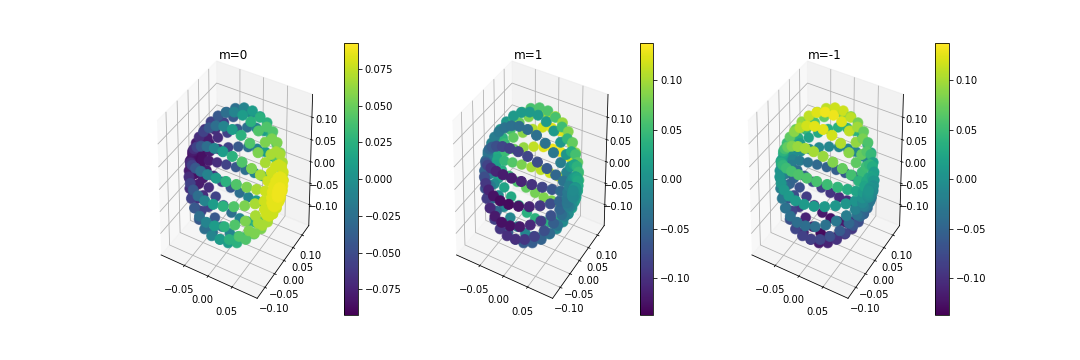
\includegraphics[width=0.99\linewidth]{equi_sh.png}
    \caption{First three eigenvectors of the equiangular laplacian}
    \label{fig:equiangular_graph}
\end{figure}

Although the three eigenvectors seems to approximate well the first mode of the spherical harmonics, the embedding of the two first eigenvectors corresponding to $Y^1_0$ and $Y^1_1$ (Fig. \ref{fig:equiangular_emb_SH}) show that they cannot form a perfect sphere, thus it still is not a satisfactory approximation.

\begin{figure}[!ht]
    \centering
    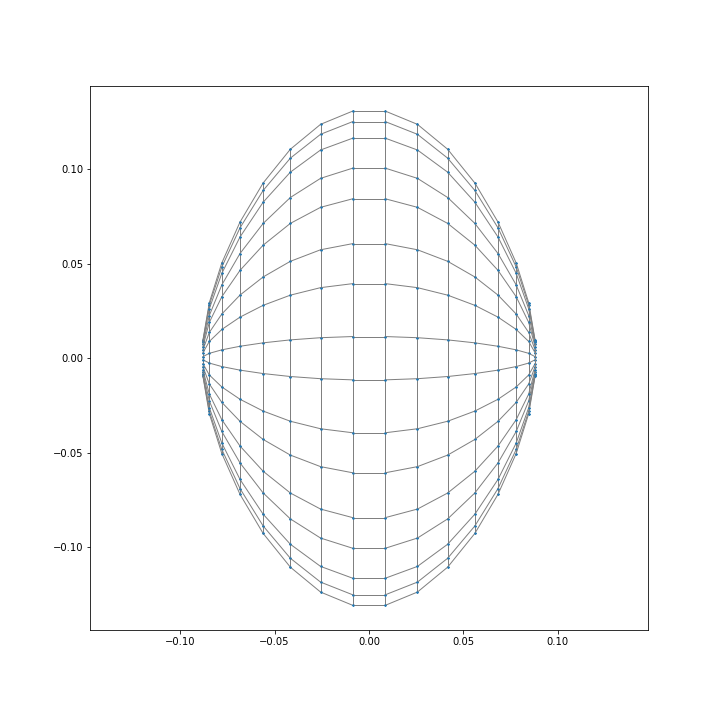
\includegraphics[width=0.5\linewidth]{figures/equi_embeded_1sh.png}
    \caption{Embedding of the two first eigenvectors of the equiangular laplacian}
    \label{fig:equiangular_emb_SH}
\end{figure}

The best case would be to use a full graph for learning. Unfortunately this Laplacian is not sparse and is too large for the GPU and Tensorflow (over 2GB limit). Furthermore, the filter will span the entire graph with only one hop, slowing the training. For these reasons, the test was done only with a 4-neighbors graph.
\subsection{Analysis}\label{sec:shrec_anal}

\subsubsection*{Results}
\paragraph*{}
The SHREC17 contest is considered from two point of views. The only differences between them is the metric used to compute the performance of the models. The first metric is a shape classification task, using the accuracy and F1-score metrics from \emph{scikit-learn}\footnote{\url{https://scikit-learn.org/}}. The second is the original shape retrieval task where the organizers provided a script to compute the necessary metrics (Precision, Recall, F1-score, mean Average Precision and Normalized Discount Cumulative Gain). Each metric is computed as an average per instance (macro) or per label (micro).

\paragraph*{}
It is seen in Fig.~\ref{fig:shrec17_overfit}, that the model learns really fast the general descriptors of the shapes, but overfits as the validation set predictions do not become better, and the model becomes more confident on the training set as the number of epochs increase. This explains why the loss on the training set keeps decreasing and the accuracy on the validation set is increasing, while the validation loss remains constant or increases steadily.

Even in this case, the results still seem to improve as the number of epochs increases, until the accuracy on the training set reaches a plateau near 100\%. Many experiments were done in order to reduce the overfit. The summary can be seen in section \ref{sec:shrec17_overfit}.

\begin{figure}[!ht]
    \centering
    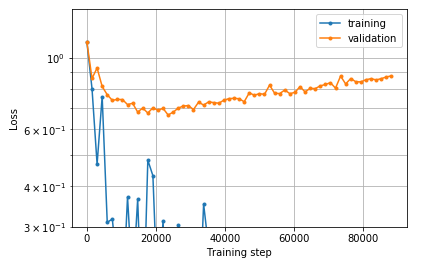
\includegraphics[width=0.8\linewidth]{plot_overfit.png}
    \caption{As the loss of the training set (blue) decreases, the loss of the validation set (orange) starts increasing, showing overfit of the model}
    \label{fig:shrec17_overfit}
\end{figure}
\paragraph*{}
However, it can be seen that using augmentation (either random translations or rotations of the models) increases slightly the performance, and the validation hits a lower plateau, with a smaller increase over time. Different augmentations were tested: 3 random translations with a maximum amplitude of 0.1, 3 random ZYZ rotations, and the combinations of them. The results of the first two is in Tab. \ref{tab:shrec17_rotequiv}. The combination, giving 6 augmented instances for the entire dataset, gives the best result, showing that the amount of data is insufficient without augmentation to learn perfectly the descriptors.

\paragraph*{}
The result of the classification task is given in Tab.~\ref{tab:SHREC17_class}. The inference speed corresponds to the time for a single instance to do a single pass of the inference, and the training speed corresponds to the time for the model to reach peak performance.
Cohen's simplified model and Esteves' model were rerun to confirm the classification metrics and the time. 

Only Cohen's original model was not fully rerun, as the original script is not provided and the complicated learning rate schedule is not given. Thus, the experiment from Cohen et al could not be reproduced exactly, and the results seem off. Indeed, the training time should be 50h and with the given hyperparameters, the real time is near 200h. The results obtained seem lower too, compared to the results Cohen reported. 

The \emph{Cohen-like} model gives similar results as the other spherical CNNs to 2 points in accuracy. The lower performance can be explained by the difference between isotropic filters (DeepSphere) and anisotropic filters (Cohen and Esteves). It is observed that DeepSphere is faster with a local filter (up to 8 times faster for the inference speed), so the \emph{Optimal} architecture can use more layers with a small impact the computational time, and reach better performance. The smaller inference time is due to a lower order for the filter ($K=4$), and the better performance, to a deeper architecture. Indeed, a single pixel has a better vision of its surroundings after each convolutional layer and the final neighborhood is close to the whole graph.

The smaller inference time for Esteves is due to the use of a local filter, and the smaller training time due to the number of epochs optimized and a greater augmentation of the dataset. And the results for the \emph{s2cnn} original seems off, due to the incorrect learning rate schedule and wrong optimizer. The publication states that the training time of the original model was 50h~\cite{cohen_convolutional_2017}.

\begin{table}[ht]
    \centering
    \begin{tabular}{l|c c r r r}
        \multicolumn{1}{l}{} & \multicolumn{2}{c}{performance} & \multicolumn{1}{c}{size} & \multicolumn{2}{c}{speed}\\
        \cmidrule(lr){2-3} \cmidrule(lr){4-4} \cmidrule(lr){5-6}
        \multicolumn{1}{l}{Method} & Accuracy & F1-score & params & inference & training \\ \hline
        Cohen \emph{s2cnn} & (73.10) & (72.86) & 1.4M & (38ms) & (65h)\\
        Cohen \emph{s2cnn\_simple} & 78.59 & 78.85 & 400k & 12ms & 32h\\
        Esteves \emph{sphericalcnn} & 79.18 & 79.36 & 500k & 9.8ms & 2h52\\ \hline
        Deepsphere \emph{Cohen-like} & 77.86 & 77.90 & 170k & 17.5ms & 9h43\\
        Deepsphere \emph{local filter} & 76.83 & 76.66 & 60k & 2.8ms & 1h37\\
        Deepsphere \emph{equiangular} & 79.25 & 79.36 & 190k & 0.98ms & 2h33m \\
        Deepsphere \emph{Optimal} & 80.42 & 80.65 & 190k & 1.0ms & 48m
    \end{tabular}
    \caption{Performance of different models (described in section~\ref{sec:shrec_anal} on SHREC17 dataset as classification task. The numbers in parentheses are got using incorrect parameters in contrast of the publication's results~\cite{cohen_spherical_2018}}
    \label{tab:SHREC17_class}
\end{table}

% \begin{table}[ht]
%     \centering
%     \begin{tabular}{l|c c r c r r}
%         \multicolumn{1}{l}{} & \multicolumn{2}{c}{performance} & \multicolumn{2}{c}{size} & \multicolumn{2}{c}{speed}\\
%         \cmidrule(lr){2-3} \cmidrule(lr){4-5} \cmidrule(lr){6-7}
%         \multicolumn{1}{l}{Method} & Accuracy & mAP & params & features & inference & training \\ \hline
%         % Cohen \emph{s2cnn} & (73.10) & (72.86) & 1.4M & (38ms) & (65h)\\
%         Cohen \emph{s2cnn\_simple} & 78.59 & 66.5 & 400k & $2\cdot 64$ & 12ms & 32h\\
%         Esteves \emph{sphericalcnn} & 79.18 & 68.5 & 500k & $8$ & 9.8ms & 2h52\\ \hline
%         % Deepsphere \emph{Cohen-like} & 77.86 & 65.4 & 170k & $ \sqrt{3}N_{side}$ & 17.5ms & 9h43\\
%         % Deepsphere \emph{local filter} & 76.83 & 76.66 & 60k & 2.8ms & 1h37\\
%         % Deepsphere \emph{equiangular} & 79.25 & 66.5 & 190k & 0.98ms & 2h33m \\
%         Deepsphere \emph{Optimal} & 80.42 & 68.6 & 190k & $4$ & 1.0ms & 48m
%     \end{tabular}
%     % \caption{Performance of different models (described in section~\ref{sec:shrec_anal} on SHREC17 dataset as classification task. The numbers in parentheses are got using incorrect parameters in contrast of the publication's results~\cite{cohen_spherical_2018}}
%     \label{tab:SHREC17_class2}
% \end{table}
\begin{table}
\begin{tabular}{l|c c c c c c c}
        \multicolumn{1}{l}{} & \multicolumn{4}{c}{Accuracy} & \multicolumn{3}{c}{Average Precision}\\
        \cmidrule(lr){2-5}\cmidrule(lr){6-8}
        \multicolumn{1}{l}{Method} & BG & TC & AR & mean & TC & AR & mean \\ \hline
        %Mudigonda et al. & 97 & 74 & 65 & 78.67 & - & - & - \\
        Jiang et al. & 97 & 94 & 93 & 94.67 & - & - & -\\
        Cohen et al. (S2R) & 97.3 & 97.8 & 97.3 & 97.5 & - & -& 68.6\\
        Cohen et al. (R2R) & 97.4 & 97.9 & 97.8 & 97.7 & - & -& 75.9\\ \hline
        % Deepsphere \emph{Cohen-like} & 77.86 & 65.4 & 170k & $ \sqrt{3}N_{side}$ & 17.5ms & 9h43\\
        % Deepsphere \emph{local filter} & 76.83 & 76.66 & 60k & 2.8ms & 1h37\\
        % Deepsphere \emph{equiangular} & 79.25 & 66.5 & 190k & 0.98ms & 2h33m \\
        %Deepsphere & 97.9 & 96.0 & 97.9 & 97.3 & 58.32 & 92.51 & 75.42 \\
        % DeepSphere & 98.0 & 99.2 & 97.4 & 98.2 & 62.13 & 96.91 & 79.5
%        DeepSphere & 98.2\pm 0.5 & 97.4\pm 1.1 & 97.7\pm 0.7 & 97.8\pm 0.3 & 58.88\pm 3.17 & 95.41\pm 1.51 & 77.15\pm 1.94
    \end{tabular}
    \caption{Climate pattern segmentation accuracy (\%) for BG, TC
and AR classes plus mean accuracy, average precision for positive classes and mean as well.}
\end{table}

% print(np.mean([98.0037, 99.022, 97.9, 98.05081171, 99.446252, 98.4880191]), np.std([98.0037, 99.022, 97.9, 98.05081171, 99.446252, 98.4880191]))
% print(np.mean([99.1810, 97.2590, 96.0, 97.30511752, 94.76495, 97.87860756]), np.std([99.1810, 97.2590, 96.0, 97.30511752, 94.76495, 97.87860756]))
% print(np.mean([97.4420, 96.7346, 97.9, 98.63355243, 88.89887, 98.15007994]), np.std([97.4420, 96.7346, 97.9, 98.63355243, 88.89887, 98.15007994]))
% print(np.mean([97.6721, 98.2089, 97.3, 97.99649, 94.37, 98.1722355306912]), np.std([97.6721, 98.2089, 97.3, 97.99649, 94.37, 98.1722355306912]))
% print(np.mean([0.62133, 0.62133, 0.5832, 0.58263467, 0.535618, 0.63429263, 0.61089104]), np.std([0.62133, 0.62133, 0.5832, 0.58263467, 0.535618, 0.63429263, 0.61089104]))
% print(np.mean([0.96912, 0.96023, 0.9251, 0.95913965, 0.956805, 0.960448, 0.96220453]), np.std([0.96912, 0.96023, 0.9251, 0.95913965, 0.956805, 0.960448, 0.96220453]))
% print(np.mean([0.79522, 0.79078, 0.7542, 0.77089, 0.74621, 0.79737, 0.786547789]), np.std([0.79522, 0.79078, 0.7542, 0.77089, 0.74621, 0.79737, 0.786547789]))

\paragraph*{}
In the case of the shape retrieval task, an additional loss was added to improve the performance and reduce the overfit. Inspired by Esteves~\cite{esteves_learning_2017}, the triplet loss promotes smaller distance between similar results and penalizes the distance between instances that are different. Thus, only the \emph{Optimal} architecture had this extra loss.

\paragraph*{}
The result of the retrieval task is given in table \ref{tab:SHREC17_retriev}. These metrics are provided by the official script of the competition\footnote{\url{https://shapenet.cs.stanford.edu/shrec17/code/evaluator.zip}}. In addition to others SCNNs, the winners of the SHREC17 competition are added to compare with state-of-the-art task-specific models. The \emph{s2cnn} original are the original publication results of Cohen's work \cite{cohen_spherical_2018}, for the reasons explained earlier.

Once again, Deepsphere reaches similar results as the others SCNNs, with lower performance for \emph{Cohen-like} and \emph{local filter}, and slightly better performance for the \emph{Optimal} model.

\paragraph*{}
Concerning the \emph{equiangular} run, even using the \emph{Optimal} architecture, the results are worse than the others. This shows that the chosen equiangular graph is not good enough, as expected from Fig.~\ref{fig:equiangular_emb_SH} and not as equivariant to rotation as the HEALPix graph. However, despite the disadvantages of the equiangular sampling, results are close to the other Deepsphere models. This may be explained by the fact that the low frequencies are the most important ones, in order to reach good results for this task, and this graph only approximates well the first order. Please refer to Martino Milani's work for further precisions \cite{milani_about_nodate}. If a better graph could be constructed for this model, similar performance as the HEALPix graph could be expected.

\begin{table}[ht]
    \centering
    \begin{tabular}{l|c c c c|c c c c}
     & \multicolumn{4}{c|}{micro (label average)} & \multicolumn{4}{c}{macro (instance average)} \\
    Method & P@N & R@N & F1@N & mAP & P@N & R@N & F1@N & mAP \\ \hline
    Furuya DLAN & 0.814 & 0.683 & 0.706 & 0.656 & 0.607 & 0.539 & 0.503 & 0.476 \\
    Tatsuma ReVGG & 0.705 & 0.769 & 0.719 & 0.696 & 0.424 & 0.563 & 0.434 & 0.418\\ \hline
    Cohen \emph{s2cnn} & 0.701 & 0.711 & 0.699 & 0.676 & - & - & - & - \\
    Cohen \emph{s2cnn\_simple} & 0.704 & 0.701 & 0.696 & 0.665 & 0.430 & 0.480 & 0.429 & 0.385\\
    Esteves \emph{sphericalcnn} & 0.717 & 0.737 & - & 0.685 & 0.450 & 0.550 & - & 0.444\\ \hline
    Deepsphere \emph{Cohen-like} & 0.695 & 0.688 & 0.684 & 0.654 & 0.424 & 0.478 & 0.423 & 0.389\\
    Deepsphere \emph{local filter} & 0.684 & 0.682 & 0.676 & 0.643 & 0.410 & 0.452 & 0.398 & 0.354 \\
    Deepsphere \emph{equiangular} & 0.709 & 0.700 & 0.698 & 0.665 & 0.439 & 0.489 & 0.439 & 0.403 \\
    Deepsphere \emph{Optimal} & 0.725 & 0.717 & 0.715 & 0.686 & 0.475 & 0.508 & 0.468 & 0.428
    \end{tabular}
    \caption{Performance of different models over SHREC17 perturbed dataset as a retrieval task, using the official script of the competition. The first two models are high-scorer of the competition.}
    \label{tab:SHREC17_retriev}
\end{table}

\paragraph*{}
To summarize, the equivariance to the $3^{\textrm{rd}}$ rotation is an unnecessary price to pay, as the difference in speed is up to 40 times, and the difference in performance is small and can be counterbalanced by having a deeper model to reach similar results. The drawback of this choice is the increased computational cost, but DeepSphere is a scalable method instead of SHFT-SCNNs, thus it is still advantageous. Thus, an isotropic filter is sufficient for this task and this representation of the data.

\subsection{Further improvements}
\paragraph*{}
The spherical projection used to represent the 3D shapes is a poor representation of it, mainly due to the fact that information is missing when there are occlusions within the object, or some surface are near parallel to the ray casted. In Fig. \ref{fig:bookshelf}, there is a specific example of an object (a bookshelf in this case) with occlusions and near parallel surfaces and its representation as a spherical signal (Fig. \ref{fig:bookshelf_spherical}).

\begin{figure}[!ht]
\centering
\begin{minipage}{0.48\linewidth}
    \centering
    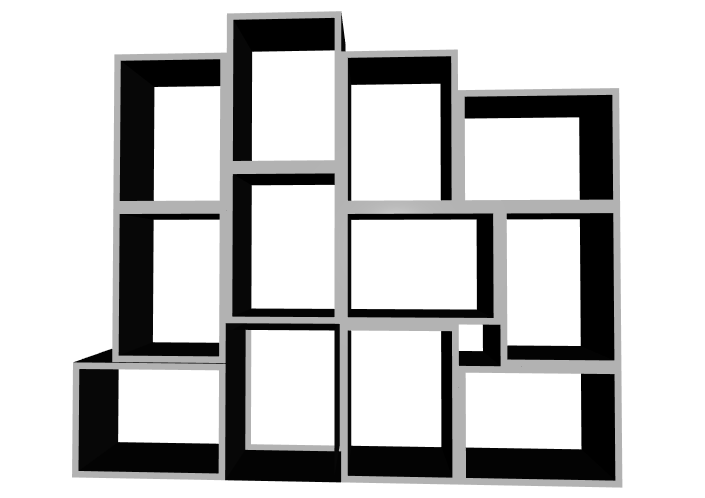
\includegraphics[width=0.8\linewidth]{bookshelf.png}
    \caption{Bookshelf shape}
    \label{fig:bookshelf}
\end{minipage}
\hfill
\begin{minipage}{0.48\linewidth}
    \centering
    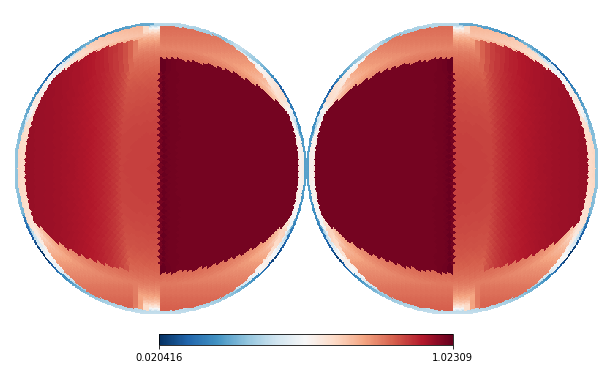
\includegraphics[width=0.8\linewidth]{bookshelf_spherical.png}
    \caption{Back view (left) and front view (right) of the spherical signal of the bookshelf obtained by ray-casting the distance from the ray to the first intersection.}
    \label{fig:bookshelf_spherical}
\end{minipage}
\end{figure}

\paragraph{}
A new possibility to represent the data is to use a multi-view CNN, as proposed by Esteves~\cite{esteves_equivariant_2019}. Each signal pixel is the resulting descriptor given by a classical CNN applied on the projected view from a certain perspective. These projected views can capture more information than a simple spherical projection.

Another possibility is to create a graph directly from the vertices of the mesh model. The problem is that the graph is not constant anymore and we do not know how the model will learn the filters. It would not be a signal on graph classification anymore, but more a graph classification task, where the goal is to identify the graph directly.

\section{In-depth investigations}
\paragraph*{}
In this section, further investigations about the behavior of DeepSphere are done in order to understand better the previous results.

\subsection{Features influence}
\paragraph*{}
As the model is clearly overfitting, many operations are tested in order to reduce the overfit. One of these operations is to reduce the number of features, keeping only the most important one, the distance feature. All the other features can be computed from this one only. One of the hypotheses is that too many features prevented the model to learn simpler correlation.

\begin{figure}[!ht]
    \centering
    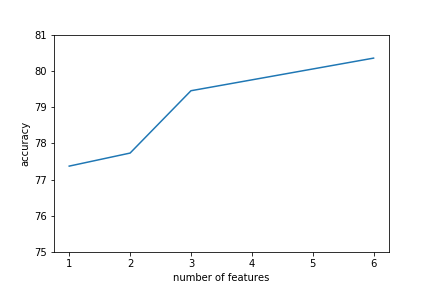
\includegraphics[width=0.5\linewidth]{figures/feat_inf.png}
    \caption{Accuracy (in percents) compared to the number of features}
    \label{fig:feat_influece}
\end{figure}
Keeping the fixed architecture \emph{Optimal} and fixed number of epochs, the number of features changed, and the resulting accuracy is shown in Fig. \ref{fig:feat_influece}. One can notice that most of the necessary information can be retrieved only by the first feature, the distance to the sphere. The influence of the remaining features is therefore small.
However, this difference is non negligible, and the addition of the cosine information (feature 3) seems to help more than the others.

\subsection{Sampling Density}
\paragraph*{}
To see where the important information needed for the neural network lies in the spectral domain, it is important to experiment with the sampling density. As the other models used only a low sampling density, it was assumed that it was due to their high computational cost. As DeepSphere is faster, sampling projections with higher density can more easily be used. The information given by a discrete sampling increases with its density, and similar to Shannon theorem, the maximum frequency that can be represented on the sampling scheme increases as well. But in the graph \ref{fig:samp_density_influece} one can see that the main information learned by the model lies in the low frequency. Indeed, even with a density of $N_{side}=8$, the model performs well. It's only by going as low as $N_{side}=2$ that it does not converge anymore.
% \todo[inline]{redo experimentation for numbers}
\begin{figure}[!ht]
    \centering
    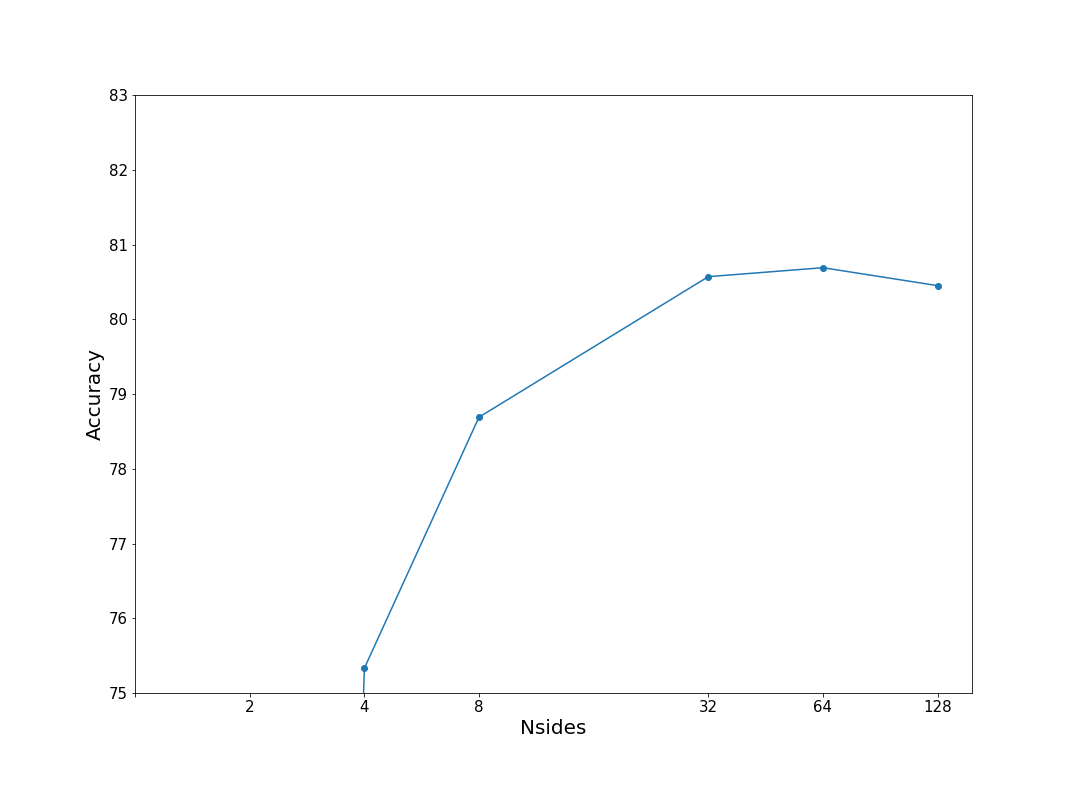
\includegraphics[width=0.7\linewidth]{density_plot.png}
    \caption{Accuracy (in percents) represented for different values of the sampling density $N_{side}$}
    \label{fig:samp_density_influece}
\end{figure}
The maximum frequency (spherical harmonic order) $l_{max}$ for HEALPix is given by $3*N_{side}-1$, where discretized spherical harmonics are still linearly independent\footnote{\url{https://healpix.sourceforge.io/pdf/facilities.pdf}}. So the maximal frequency increases with the density $N_{side}$.

\subsection{Rotation Equivariance}\label{sec:shrec17_equivariance}
\paragraph*{}
In order to see if the equivariance to rotation was sufficient for the given task, or if it was needed to learn the correct equivariance with data augmentation, another experimentation was done. For the same architecture, the model learned from two different datasets. The first was augmented with three random translations while the rotation is kept the same for every instance, resulting in the objects not being in the center of the sphere anymore. The second dataset was augmented with three random rotations. Thus, the two datasets have the same number of instances.
It was then tested on the test sets processed with the same manner. The results can be seen in the Table \ref{tab:shrec17_rotequiv}.

A sampling density of $N_{side}=32$ was chosen.
\begin{table}[!ht]
    \centering
    \begin{tabular}{c|c|c|c|c}
         & NR/NR & R/NR & R/R & NR/R  \\ \hline
Accuracy & 79.57 & 79.26 & 79.25 & 79.82 \\\hline
mAP@N    & 67.1 & 67.0 & 67.5 & 67.4
    \end{tabular}
    \caption{Performance of DeepSphere (accuracy and mean average precision in percent) in X/Y configuration, trained on X dataset while tested on Y dataset. R corresponds to rotation augmentation and NR corresponds to translation augmentation.}
    \label{tab:shrec17_rotequiv}
\end{table}
It can be concluded that the model is sufficiently equivariant to rotation for this task, as the results are similar, whichever the conditions.

\subsection{Use of more equivariant graph}
\paragraph*{}
Following the work of Martino Milani, a more precise rotation equivariant graph has been constructed \cite{milani_about_nodate}. The experiments were rerun with the better HEALPix graphs and the results can be seen in Table \ref{tab:martino_shrec17}. As seen in the section~\ref{sec:shrec17_equivariance}, the previous graph is sufficiently equivariant to rotation for this specific task, it is therefore no surprise to not to see any improvement with an improved graph. Indeed, in the first graph, the first orders of the spherical harmonics are well approximated, and higher orders seem to diverge more, so only high frequency signal would suffer from such a graph. In this task, it was shown experimentally earlier that the important frequencies are the lowest ones, and the model will not benefit from a better discrimination of the higher frequencies. 

\begin{table}[]
    \centering
    \begin{tabular}{c|ccc}
          & old graph & new kernel size & new graph \\ \hline
accuracy  & 82.23 & 82.45 & 82.76
    \end{tabular}
    \caption{Performance with better equivariance}
    \label{tab:martino_shrec17}
\end{table}

\subsection{Preventing overfit}\label{sec:shrec17_overfit}
As shown earlier, the model overfits the data, and several methods are tested to reduce this effect. The resulting accuracy on the validation set is regrouped in Table \ref{tab:shrec17_overfit}. Without any method to prevent overfitting, the accuracy is $81.8\%$.
\paragraph*{Regularization}
To prevent the apparition of a too complex model with overly large parameters, L2-regularization is used. In this specific case, a complex model is preferrable as the accuracy drops by 1 point.
\paragraph*{Dropout}
Another classical method is to apply dropout on the fully-connected layer. This prevents this layer to become too specific. This method shows no clear improvement in the performance.
\paragraph*{DropFilter}
The same idea can be applied on the convolutional layers by dropping whole filters instead of neurons. Again, it is apparent that this method is not beneficial to the model. The layers are not trained long enough to become too specific.
\paragraph*{Triplet Loss}
As explained earlier, an additional loss presented first by Esteves was added to increase the performance for the retrieval task. However, the gain is negligible.
\paragraph*{Data augmentation}
Different data augmentation are tested. The first is the addition of a random Gaussian noise 
with $\sigma=0.1$ to the spherical signal. This deviation is too big and the results remain stable. Another problem is that the data is too large too compute random noise on the fly, and only five noise configurations are computed before training.

Finally, the data was augmented using random translations and rotations. The rotation is not necessary, but reused from the section \ref{sec:shrec17_equivariance}. After using 6 different configurations for each instance, the effects of overfitting are less present as the validation loss has a slower increase over time, and the final accuracy is slightly higher. It can be assumed that if more configurations were used, the performance would increase even more.

\paragraph*{Summary}
No method prevents the overfitting in this case. Only the triplet loss and the data augmentation are able to reduce its effect. It may be due to the fact that the dataset is too small and a larger population is needed to find correct representations of shape descriptions.

\begin{table}[!ht]
    \centering
    \begin{tabular}{c|cccccc}
 & $\varnothing$ & Regularization & Dropout & DropFilter & Triplet Loss & Data aug.\\ \hline
Accuracy & 81.8 & 80.7 & 82.4 & 81.5 & 82.5 & 83.4\\
    \end{tabular}
    \caption{Different methods preventing overfit}
    \label{tab:shrec17_overfit}
\end{table}
% \section{Influence of sampling}
% \subsection{dataset}
% Projection of images, 3D objects on different parts of sphere
% Dataset1: projected on equator
% Dataset2: project on pole
% Dataset3: combination of D1 and D2
% Train on D1, D2 and D3 and see how they react on each dataset

% Not done, and will maybe not be done. different graph each time. Not change from mock dataset such as Spherical-MNIST

\section{Classification task - ModelNet40}\label{task:mn40}
\subsection{Task presentation}
\paragraph*{}
The ModelNet40 dataset is very similar to the SHREC17 dataset, as it is a collection of 3D CAD models. The only differences are the number of classes and the total number of instances. There are only 40 common classes instead of 55, and about 80\% less instances, making the classification task harder as it was shown that the SHREC17 dataset was not large enough for the model to grasp perfectly the shape descriptors.

\paragraph*{}
Is it is a similar task as section \ref{sec:shrec17}, the preprocessing is kept the same, and there is no need to redo an intensive study of the task, and the decision was taken to reuse the same architecture. Additionally, publicated results on this tasks could be used for comparison with DeepSphere.

There are two different datasets, a manually aligned and a randomly rotated version. For the same reasons as for SHREC17 task, the perturbed dataset is chosen.

\subsection{Other spherical models}
\paragraph*{}
The first spherical CNN to compare to is Esteves \emph{sphericalcnn}, that is the same as for SHREC17 retrieval task. It is not specified which dataset is chosen, but it is more likely that the perturbed version has been used. However, in his latest study \cite{esteves_equivariant_2019}, the aligned version was used to compare more easily with other publications.

Again, equiangular is the sampling scheme chosen and  augmentation was used to increase the performance and prove the equivariance to rotation. The model learns first on random rotation around $z$ (euclidean coordinate), and is tested on random $SO(3)$ rotations. A drop in performance for this test can be seen. This was attributed to the problem of the equiangular sampling.

\paragraph*{}
Jiang uses the aligned dataset because inherently it is not equivariant to rotation. Indeed, Jiang argued that, for classification problems, the orientation is important. For example with omnidirectional images with the gravity, and planetary signals with the axis of rotation \cite{jiang_spherical_2019}.
Additionally, Cohen's \emph{s2cnn} was used to have more comparison. But no augmentation was used and it was obviously not tested with random rotation disturbances.

\subsection{Analysis}
\paragraph*{}
DeepSphere \emph{Optimal} model is reused for the two configurations of the experiment: The first configuration being (x/x), with no augmentation during training, and the only difference being the non aligned dataset, explaining a little drop in performance. The second configuration includes augmentations only around the Z-axis (z) and with random $SO(3)$ rotations (SO3) for the test set. The notation (X/Y) simply shows that the model was trained on X and tested on Y. In this specific case, only 3 different random configurations are used for augmentation.
The resulting accuracy can be observed in Table \ref{tab:mn40_results}

\paragraph*{}
Even if it was not tested, it is expected that Jiang would perform poorly with rotation perturbations, as it is not equivariant nor invariant to rotation. Otherwise, it outperforms other spherical CNNs with the aligned dataset.

\begin{table}[!ht]
    \centering
    \begin{tabular}{c|cccc}
         &  x/x & z/z & SO3/SO3 & z/SO3 \\ \hline
Cohen & 85.0 & - & - & - \\
Jiang & 90.5 & - & - & - \\
Esteves \emph{scnn} & - & 88.9 & 86.9 & 78.6 \\
%Esteves \emph{MVCNN} & 94.69 & - & - & - \\
DeepSphere & 87.8 & 86.8 & 86.7 & 76.9
    \end{tabular}
    \caption{Accuracy (in percent) on test set, for different models. The x dataset has no augmentation, the z dataset is augmented with rotation around Z-axis, and SO3 with ZYZ rotations.}
    \label{tab:mn40_results}
\end{table}

\paragraph*{}
Again, similar results can be observed with only a drop of 1 point in accuracy, potentially due to the the isotropic filter. But the same drop in performance as Esteves when using SO3 test set can be observed, even using a more uniform sampling such as HEALPix. Thus the origin of this drop might be elsewhere than in the sampling. It is still possible that the sampling HEALPix, being iso-latitude, has a more faithful representation for rotation in Z (latitudes remain the same), but other possibilities must be explored.

Additionally, the behaviour is the same as SHREC17, where the model learns quickly (about 10 epochs) the shape descriptor and start overfitting.

% Furthermore, adding more augmentated data increased the result until
\paragraph*{}
A first hypothesis was that the equivariance to rotation is not good enough for this task. Thus, the evolution of the logits (probabilities to belong to each of the 40 classes) for different is observed. First, a discrete rotation of the sampling is made to prove that the theory is correct and the model is correctly implemented. A HEALPix map has discrete rotations around Z ($\phi$) every 90\degree and around X or Y ($\theta$) every 180\degree. Indeed, the empirical result show that these specific shifts of the map give the exact same result, so the model is exactly equivariant to discrete rotation and approximately equivariant for other rotation.

Next, random $SO(3)$ rotations are performed and the evolution of the logits are seen in Fig. \ref{fig:mn40_logits}. The x-axis represents the 40 classes, and the y-axis is the output of the softmax, the probability for the shape to belong to a specific class. A specific instance of a class with low accuracy is chosen (in this case, a 'desk'), and the model is trained on the dataset with Z-axis rotation augmentation.
The blue dots correspond to the response of a model trained on original orientations, and the other three colors corresponds to models that learned with three $SO(3)$ random rotations.

When two classes have a high probability to be chosen, the small perturbations added by a non-discrete rotation are sufficient to change the final decision.
\begin{figure}[!ht]
    \centering
    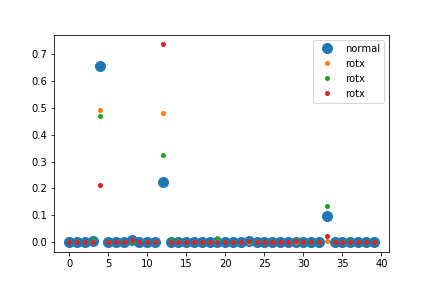
\includegraphics[width=0.7\linewidth]{figures/logits_change.png}
    \caption{logits (probabilities to belong to each of the 40 classes) evolution for different rotation configuration for indistinguishable class}
    \label{fig:mn40_logits}
\end{figure}
\paragraph*{}
Upon further investigation, some 3D shapes are only surfaces and have no spherical projection. Adding the fact that some shapes have a poor spherical representation (see for example Fig. \ref{fig:bookshelf_spherical}), the model cannot learn the correct descriptors to distinguish the classes.
% plant\_0338 is flat and cannot be ray casted.
% plant\_0078
\paragraph*{}
Furthermore, some classes are indistinguishable with the level of information the model is able to grasp and accuracy will vary greatly between them. This can be seen in Fig. \ref{fig:mn40_conf_matrix}, where the confusion matrix of the Z test dataset is shown. 
Some very distinguishable classes such as 'airplane' and 'laptop' have a very high accuracy because they are very different from the rest of the classes. Even if the test is done with the SO3 dataset, the accuracy stays the same (see Fig. \ref{fig:mn40_logits_airplane}). But other classes such as 'plant', 'flower pot' and 'vase' are indistinguishable and have a poor accuracy (between 30 and 60 \%) and testing on the SO3 dataset only worsens this accuracy (a decrease of 35 points can be observed). This shows that the model is still unsure how to classify correctly the shapes, and the very similar classes do not help in this case. Even trying to increase the training time for the model to be more confident does not change the behaviour (increasing the number of epochs by three).

\begin{figure}[!ht]
    \centering
    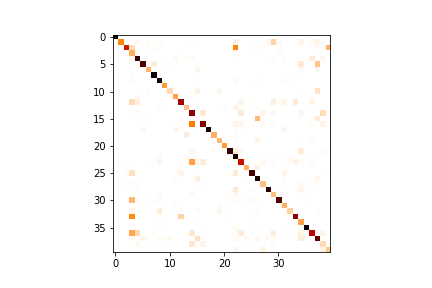
\includegraphics[width=0.7\linewidth]{figures/conf_matrix.png}
    \caption{confusion matrix of test set}
    \label{fig:mn40_conf_matrix}
\end{figure}


\paragraph*{}
Thus, it is possible that there are not enough samples to learn the indistinguishable classes. Sampling density $N_{side}$, the number of features and the type of graph were changed to see the differences. However, there were no noteworthy differences observed. Even the more accurate graph in respect to the equivariance to rotation did not change the results.


\begin{figure}[!ht]
    \centering
    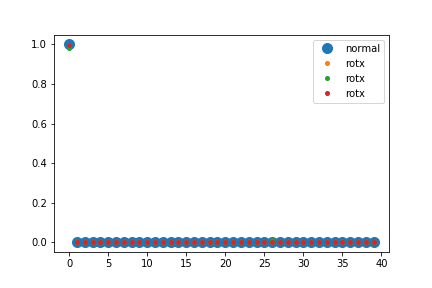
\includegraphics[width=0.7\linewidth]{figures/logits_change_airplane.png}
    \caption{Logits evolution for different rotation configuration for distinguishable class. The invariance is perfect in this case}
    \label{fig:mn40_logits_airplane}
\end{figure}

\paragraph*{}
The problem may be due to the spherical representation, where information is lost, and the dataset being too small for the model to comprehend the features correctly.
Using augmentation (adding random $SO(3)$ rotations) during training, the drop in performance when testing on SO3 dataset could be reduced drastically, but the performance when testing on Z dataset is not increased.

\section{Dense regression - GHCN-daily}\label{task:GHCN}
\subsection{Dataset presentation}
\paragraph*{}

The goal is to build an irregular, sparse and non-uniform graph around the world with every node corresponding to a weather station, and the graph signals to the different measurements. To be useful, the graph must be as large as possible. If the graph represents a too small region, the curvature of the Earth will not be visible and the resulting graph will not differ from a planar one, and it would make no sense to use a spherical CNN. An example of a graph using all the weather stations around the world is shown in Fig. \ref{fig:world_graph}.

The data of interest for this study is chosen from 2010 to 2014, corresponding to 1826 days. The different measurements are described in the README of the dataset\footnote{\url{https://www1.ncdc.noaa.gov/pub/data/ghcn/daily/readme.txt}}.

In all the cases, no irregular graph sampled densely over the continents can present the equivariance to rotation property. It is not the purpose of this part of the study, as were are interested in the flexibility of DeepSphere. In any case, the $S^2$ symmetry group does not seem present in this task. The weather is not the same between the poles and the equator, and there may be differences between oceans and continents. The only meaningful rotation might be Z due to the axis of rotation of the Earth.

Regarding the isotropic filter, it may not be a hindrance if one is only interested in finding different regions of specific weather (e.g. "blobs" of high precipitation).

\paragraph*{}
For the current problem, only the most represented measurements (minimum and maximum temperatures, precipitation and snow fall) should be chosen to have the largest graph. Any other measurements are not represented enough over the globe (less than 10'000 weather stations during the interval of interest).
On top of that, there are lots of abnormal data and impossible outliers, such as minimum temperature higher than maximum temperature or far outside possible ranges. Fortunately, the dataset provides a quality flag that lets one know if the data might be corrupted or has problems. Thus, any data that raised a quality flag was removed.

\subsubsection{Find a task}
\paragraph*{}
This dataset was a perfect opportunity to prove the flexibility of DeepSphere, as the weather stations did not form a great regular sampling (higher concentration in some countries, and almost no sample points over oceans), and interpolation over the whole sphere does not make much sense because the data points are too far away from each other in less populated areas. At the time of the study, no one used this dataset and no specific task was obvious enough for a deep learning problem. So one of the first steps is to find a specific task to demonstrate the advantage of DeepSphere.

The main tasks considered are global classification (e.g. classify the weather on the whole globe such as find the season or era), global regression (e.g. prediction of a specific variable, such as time), segmentation or dense classification (e.g. find a class for each node, such as weather type) and dense regression (e.g. predict a specific variable from the other features).

Global tasks are not really useful nor complicated in this case therefore this possibility was immediately dropped. Dense classification and segmentation were also dropped because there were not enough labels and no information to apply ourselves the other labels, and a great coverage could not be constructed. Only dense regression tasks are doable realistically, using already known features as variables to predict.

\paragraph*{}
As only few features are sufficiently present, only a few tasks were possible:
\begin{enumerate}
    \item Find the maximum temperature from the minimum temperature
    \item Find precipitation from temperature (max and min)
    \item Find snowfall from temperature and precipitation
    \item Find temperature at day T from N days before
    % \item Find any other features from location and time only.
\end{enumerate}
\paragraph*{}
The first task does not have a great meaning and is not really useful. For the second, although interesting, it does not yield compelling results as there does not seem to exist a great correlation between these features.
The third yields similar results as the previous one. The fourth seems to be the most promising task, although we can only find statistical relations between different days, and not actually predict the future.

\paragraph*{}
Different features were added in the hope of increasing the performance, such as the latitude and altitude of the weather station, and the time of the year (approximated by a sinus over the 366 days to represent the periodicity of the seasons). These additional features were added as there seems to be a correlation between the time of the year, the location of the place and the temperature. Indeed it is warmer in summer in the northern hemisphere for example.

\paragraph*{}
To augment the data or have a larger graph, one idea was to take a superset of weather stations that had a majority of measurements (over 75\%  during the interval of interest) for the chosen features, and to inpaint (using regression Tikhonov\footnote{\url{https://github.com/epfl-lts2/pygsp/blob/master/pygsp/learning.py}} on the given graph) the missing data. These will be used for the learning and results will be masked for the computation of the loss and final response. The main problem is that the regression will give a smooth signal on the missing nodes, using the graph structure that is used for the learning afterwards. Basically, it is counterproductive and forces the model to learn a smooth response at the end.

Practically, a mask of the missing values is given as feature for the model so it knows where the real values are. The inpainted values are ignored for the back-propagation part of the learning (the loss of the masked values are forced to 0). Similarly, for the response of the model, the masked values return NaN.

\subsection{Implementation}
\paragraph*{}
A new graph must be constructed as the sampling is irregular and the HEALPix graph is useless in this case. The graph nodes correspond to the weather stations, represented by their latitude and longitude on Earth. To connect the nodes, a knn-graph\footnote{\url{https://pygsp.readthedocs.io/en/stable/reference/graphs.html\#pygsp.graphs.NNGraph}} is used, with the number of neighbors for each node a hyperparameter. The first number of neighbours is fixed at 5 arbitrarily. Thus, the weight matrix is a standard heat diffusion kernel using the euclidean distance. There is an example of a graph using only USA weather stations in Figures \ref{fig:USA_graph_front} and \ref{fig:USA_graph_sphere}. Figure~\ref{fig:USA_graph_up} shows that the curvature of the Earth is significant even using only this country.

Each day corresponds to a new spherical signal represented by the chosen features.

\begin{figure}[!ht]
    \centering
    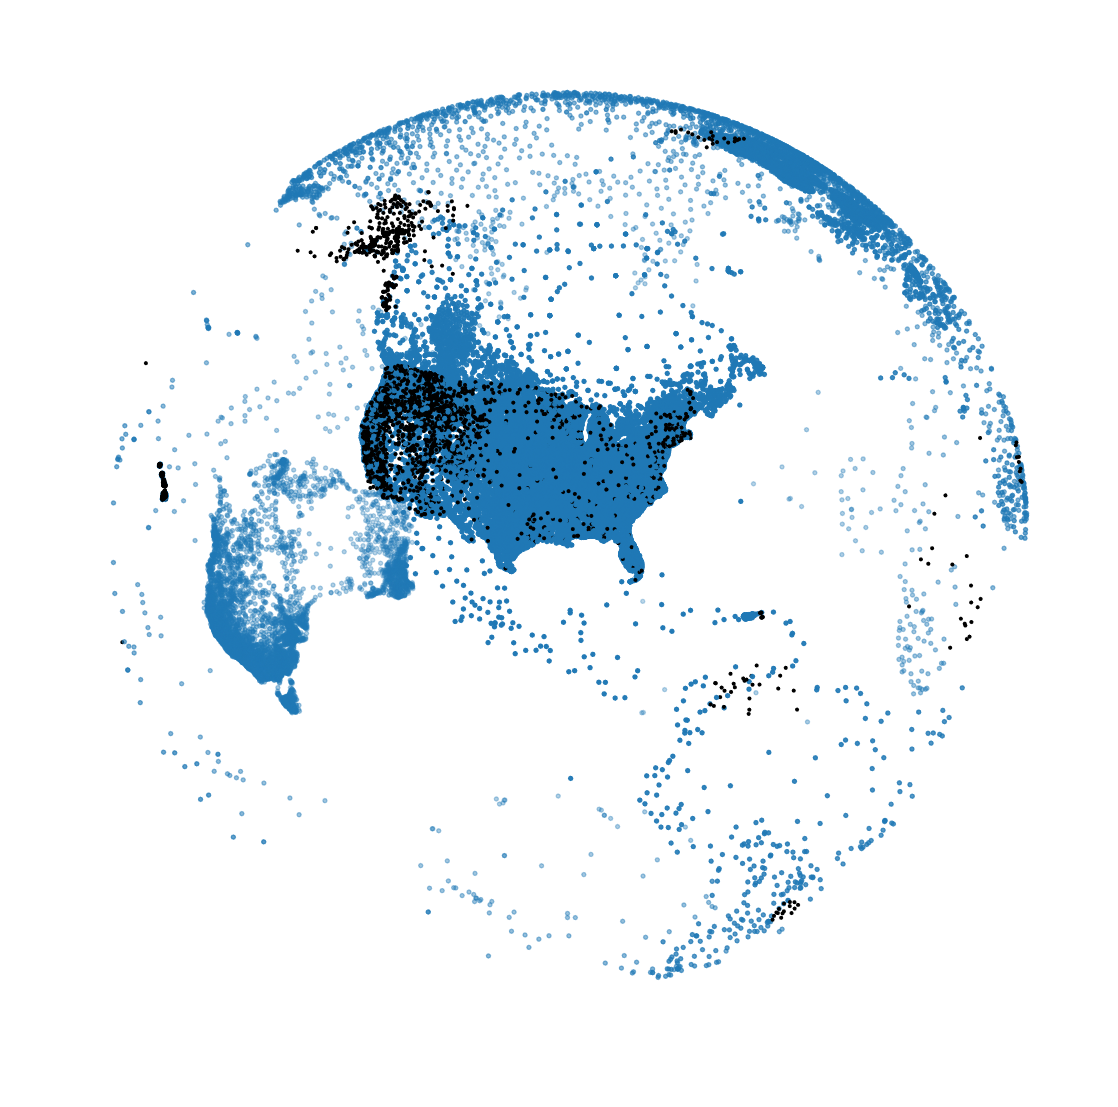
\includegraphics[width=0.5\linewidth]{world_graph_USA.png}
    \caption{Graph of the world weather stations}
    \label{fig:world_graph}
\end{figure}

\begin{figure}[!ht]
\centering
\begin{minipage}{0.8\linewidth}
    \centering
    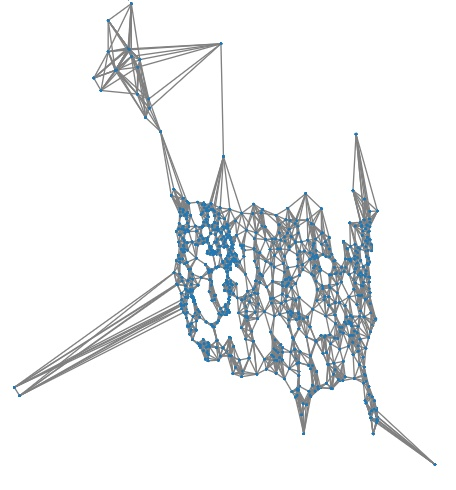
\includegraphics[width=0.7\linewidth]{USA_temp_2.jpg}
    \caption{Front view of the graph for USA weather stations only}
    \label{fig:USA_graph_front}
\end{minipage}\\
\begin{minipage}{0.4\linewidth}
    \centering
    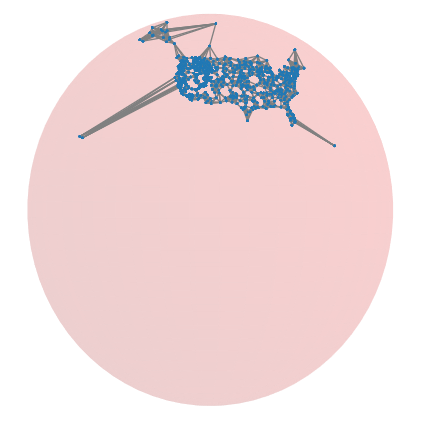
\includegraphics[width=0.99\linewidth]{USA_temp.png}
    \caption{Graph of the USA weather stations represented on a spherical Earth}
    \label{fig:USA_graph_sphere}
\end{minipage}
\hfill
\begin{minipage}{0.48\linewidth}
    \centering
    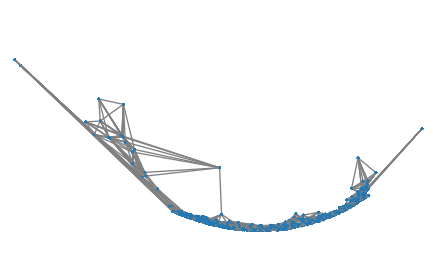
\includegraphics[width=0.99\linewidth]{USA_temp_3.png}
    \caption{View showing the curvature of the Earth as derived from the graph for USA stations only}
    \label{fig:USA_graph_up}
\end{minipage}
\end{figure}


\paragraph*{}
For the architecture of DeepSphere, no pooling is used. Indeed, there is no rule for pooling a graph with an irregular, non-hierarchical sampling. And to keep the irregularity of the sampling, the combinatorial Laplacian of the graph is used.

An MSE loss is chosen for the regression task, with an RMSprop Optimizer (decay of 0.9 and momentum of 0) and a constant learning rate of $10^{-3}$.
The resulting architecture is:
$$ NN = GC_1 \circ (ReLU \circ BN \circ GC_{100}) \circ (ReLU \circ BN \circ GC_{100}) \circ (ReLU \circ BN \circ GC_{50}). $$
The number of feature maps is arbitrarly chosen. The last one is the number of parameters to be found by the regression, so in this case just one. The order of the filters $K$ is chosen to remain fixed for all layers, but considered as a hyperparameter to change too.
A batch size of 64 is used due to the small graph and the model is run for 250 epochs.

The interval of time is separated in two parts. The training set corresponds to 70\%, so three years and a half. The remaining 30\% are the test set.

\subsection{Analysis}
\paragraph*{}
The metrics chosen to estimate the performance of the model are again computed with \emph{scikit-learn}. They are Mean Absolute Error, Mean Relative Error to observe if the predictions seems off, and R2 score to observe if the predictions are better than the mean.

\paragraph*{}
A first thing to do is to see the evolution of the performance in respect to the number of neighbors in the knn-graph ($N$), and the order of the graph filter ($K$). All runs are trained for the same number of epochs.
For a fixed $K$ of 5 (and number of previous days of 5), the performance of future temperature prediction seems to increase with the number of neighbors (Tab. \ref{tab:knn_temp}). A hypothesis is stated in the following section. The same operation was done with the precipitation task (Tab. \ref{tab:knn_prec}).

\begin{table}[!ht]
    \centering
    \begin{tabular}{c|cccc}
neighbour & MSE & MAE & R2 & batch time \\ \hline
        1 & 9.55 & 2.27 & 0.90 & 0.33s\\
        5 & 8.33 & 2.14 & 0.91 & 0.35s\\
       10 & 7.97 & 2.09 & 0.92 & 0.46s
    \end{tabular}
    \caption{Evolution of performance with different KNN-graph for the temperature task}
    \label{tab:knn_temp}
\end{table}

\begin{table}[!ht]
    \centering
    \begin{tabular}{c|cccc}
neighbour & MSE & MAE & R2 & batch time \\ \hline
        1 & 41.58 & 2.87 & 0.11 & 0.22s\\
        5 & 38.25 & 2.77 & 0.15 & 0.27s\\
       10 & 43.86 & 3.07 & 0.12 & 0.32s
    \end{tabular}
    \caption{Evolution of performance with different KNN-graph for the precipitation task}
    \label{tab:knn_prec}
\end{table}

In conclusion, when the convolutions over a pixel use fare separated neighbors, the performance drops as there is no more significant influence outside of the direct neighborhood. Additionally, a denser graph will cause an increase in inference time for the same hyperparameters. Based on this, a $N$ of 5 is chosen for the precipitation task and 10 for the future temperature task.

The filter order $K$ will be further investigated in the future temperature prediction task.

\subsubsection{Precipitation task}
\paragraph*{}
The range of temperatures is within [-53.3, 41.7] for the minimum and within [-47.2, 53.9] for the maximum. The range of precipitation is [0, 415] mm, with a mean of 2.3mm, showing that most of the data is close to 0mm.

The number of weather stations in the minSet, the set containing nodes having measurements for the whole interval of interest, is 1085 and span the USA and a part of Europe. The superSet, the set containing nodes that have at least 75\% of measurements during the interval, has 9728 nodes.

But there is a problem with the inpainting problem. As all the signals are treated separately, some abnormal values appear. Indeed, as the different features such as minimum temperature and maximum temperature are separate and there is no temporal information during the Tikhonov regression, minimum temperature higher than maximum temperature, and changes over 30\degree in one day is observed. Thus such information must not be learned.

\begin{figure}[!ht]
    \centering
    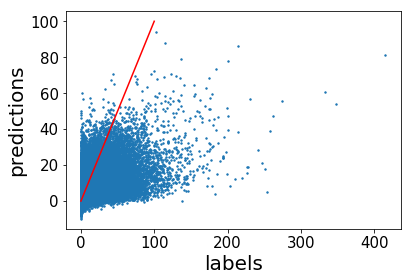
\includegraphics[width=0.5\linewidth]{figures/prec_reg_results.png}
    \caption{Predictions over true labels}
    \label{fig:prec_reg_res}
\end{figure}

It can be seen in Fig. \ref{fig:prec_reg_res} that the model does not really perform better than random guessing, and that the outliers are generally ignored, resulting in predictions around the mean.

\paragraph*{}
Without the additional features, so with only the temperature information, the model cannot find any relation, and the validation loss remains constant with some random spikes. So the model does not perform better than a random guess.

But even adding the new features does not improve the performance. The only change is that there are no more random spikes and the gradients are much smaller. Seeing the results in Tab. \ref{tab:prec_metrics}, the mean absolute error is about 3 mm of precipitation and seems low in respect to the interval, but the mean relative error is too large, showing that there are only few big values that are ignored. And thus the model only predicts the mean, as specified by the r2 score near 0.

\begin{table}[!ht]
    \centering
    \begin{tabular}{c|cccc}
         & MSE & MAE & MRE & R2 \\ \hline
    Base features & 45.44 & 2.74 & 119 & -0.04 \\
    Additional features & 38.25 & 2.77 & 140 & 0.15
    \end{tabular}
    \caption{Validation metrics for precipitation regression}
    \label{tab:prec_metrics}
\end{table}

\paragraph*{}
The results for the snowfall task is also ignored as it is similar than the precipitation one, but with less data.

\subsubsection{Future temperature task}
\paragraph*{}
The number of weather stations in the minSet, the set containing nodes having measurements for the whole interval of interest, is 1573 and span the USA, a part of Europe and few in Australia. The superSet, the set containing nodes that have at least 75\% of measurements during the interval, has 11996 nodes.

As the goal of this task is to predict the temperature at day T, the chosen features for this task are n days [T-1, ..., T-n] before the day to predict, and the other additional features are the location and altitude of weather stations as well as the day of the year.
No additional temporal information is added, but in future application it might be interesting to apply the CNN on the temporal axis as well. The minimum and maximum temperatures are considered to behave more or less the same way temporally, and are added as two different signals per day.

So the main hyperparameters are the number of days in the features (n), the number of neighbors (fixed at 10 for this experiment) and the order of the graph filter (the number of hops seen during the convolution).

\paragraph*{}
A first hypothesis is that weather affects a whole region, so it is useful to take advantage of the locality of the data, and thus use the graph. But stations that are too much distanced won't influence each other. Thus there would be an optimal filter order where the model will not learn additional information and reduce its performance.

To prove it, a first baseline is built using the measurements from the weather stations as time series. Thus, no relation between the nodes can be constructed. Practically this corresponds to use a graph f of order 0.

It is observed that for a short time window, the temperature does not have a significant change. It is then interesting to observe if the model predicts a temperature closer to day T-1 instead of day T. This will be our second baseline.

\paragraph*{}
Another interesting point is to fix the second hyperparameter, the number of previous days features for the model. The knn-graph is already constructed with the 5 nearest neighbors, and the order of the filter is still fixed at $K$=5.

\begin{table}[!ht]
    \centering
    \begin{tabular}{c|cccc}
        ndays & MSE & MAE & R2 & batch time \\ \hline 
        2 & 8.39 & 2.14 & 0.915 & 0.46s\\
        5 & 8.13 & 2.11 & 0.917 & 0.47s\\
        10 & 8.274 & 2.13 & 0.915 & 0.48s\\
    \end{tabular}
    \caption{Evolution of performance for different number of days in feature}
    \label{tab:ndays_future}
\end{table}

The performance seems to increase with the number of previous days, but the memory increases linearly and the change is not as significant as changing the graph or the order of the filter. Finally, a number of 5 days is chosen as a compromise.

\begin{table}[!ht]
    \centering
    \begin{tabular}{c|cccc}
        order & MSE & MAE & MRE & R2 \\ \hline 
        0 & 10.88 & 2.42 & 83.8 & 0.896\\
        1 & 8.91 & 2.20 & 75.1 & 0.906\\
        4 & 8.20 & 2.11 & 73.2 & 0.919\\
        9 & 8.38 & 2.12 & 73.3 & 0.915\\
    \end{tabular}
    \caption{Evolution of performance in respect of the order of the filter}
    \label{tab:future_results}
    ~\\[1cm]
    \begin{tabular}{c|cccc}
        order & MSE & MAE & MRE & R2 \\ \hline 
        1 & 134.01 & 10.51 & 282.60 & -0.319\\
        4 & 129.48 & 10.31 & 283.29 & -0.274\\
        9 & 141.68 & 10.82 & 291.34 & -0.389\\
    \end{tabular}
    \caption{Predicting the present day (T-1) instead of the future day T}
    \label{tab:present_results}
\end{table}

\paragraph*{}
Now, the last interesting part is the influence of the order of the Tchebyshev filter. In this part, it is shown that the use of a graph is beneficial for the learning as the results (Tab. \ref{tab:future_results}) are better than the baselines, and thus the structure of the data is helping.

The baseline, where the data are considered as simple time series during the training, is the order 0. The filter sees only the current node and no neighbouring nodes. The last test is to compute the metric with the present day instead of the future day (Table \ref{tab:present_results}). This other baseline is used for proving that the model predicts effectively the next day and not a random similar day.

A limit can be seen where it is not beneficial anymore to use information from neighbors that are too far away. In our case, a drop of performance is observed when $K=10$ and the peak performance is reached with $K=5$. The final comparison shows that the model is able to predict more accurately the future than the present day, which proves that it has learned a statistical representation of the future day from previous ones.
% prédit correctement le jour actuel, et pas le lendemain

% result on testing set
% K=0, MSE=10.88 , MAE=2.42, MRE=83.8, R2=0.896, Expvar=0.896
% K=1, MSE=8.91 , MAE=2.20, MRE=75.1, R2=0.906, Expvar=0.913
% K=4, MSE=8.20 , MAE=2.11, MRE=73.2, R2=0.919, Expvar=0.921
% K=9, MSE=8.38 , MAE=2.12, MRE=73.3, R2=0.915, Expvar=0.917
% baseline learn the same day
% K=0, MSE=0.037, MAE=0.185, MRE=5.4, R2=0.9996, Expvar=0.9997
% K=1, MSE=0.042, MAE=0.152, MRE=5.8, R2=0.9993, Expvar=0.9996
% K=4, MSE=0.107, MAE=0.263, MRE=7.3, R2=0.9988, Expvar=0.9992
% K=9, MSE=0.125 , MAE=0.280, MRE=7.2, R2=0.9964, Expvar=0.9994
% test on day T rather than day T+1
% K=0, MSE=132.49, MAE=10.36, MRE=282.37, R2=-0.299, Expvar=-0.2991
% K=1, MSE=134.01, MAE=10.51, MRE=282.60, R2=-0.319, Expvar=-0.3124
% K=4, MSE=129.48, MAE=10.31, MRE=283.29, R2=-0.274, Expvar=-0.2723
% K=9, MSE=141.68, MAE=10.82, MRE=291.34, R2=-0.389, Expvar=-0.3868

\paragraph*{}
One interesting result is that knowing how the rest of the world behaves helps the learning. In other words, our architecture is more successful than just using the time series from each weather stations separately.

\paragraph*{}
Once all hyperparameters fixed, a quick ablation study of the additional features (location of nodes, and day in the year) is done, and shows that the only change is the rate of learning for the training set (1 point of MSE after 250 epochs), but the results for the testing set remains the same. Thus these features are useless and the correlation seen is grasped with the fundamental features.

\paragraph*{}
Another test to do in order to know if the model grasped more or less the behaviour of the features is to only give it the first N days, feed only the predictions afterwards, and see if there is a divergence or a correct behaviour. Even if predicting the future is completely impossible and that a weather model is needed to predict anything correctly, it is possible to learn the statistical behaviour. And thus, the predictions should be oscillating between winter and summer, even without being near than correct. This is the case for the models learned.

\begin{figure}[!ht]
    \centering
    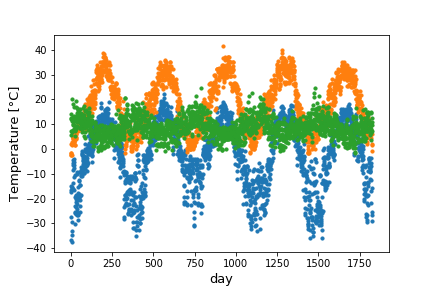
\includegraphics[width=0.6\linewidth]{figures/evolution_temp.png}
    \caption{Evolution of temperature over time for three different stations}
    \label{fig:evol_temp}
\end{figure}

% In short, the neural network is able to interpret and reproduce the past instead of predicting the true future. The advantage is that there is an underlying periodicity for these signals, and the future tends to be similar to the past, thus the model will produce acceptable results as long as the future reflects it.

\begin{figure}[!ht]
    \centering
    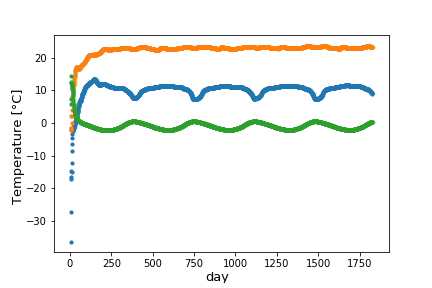
\includegraphics[width=0.6\linewidth]{figures/prediction_temp.png}
    \caption{Complete prediction of temperature over time for three different stations}
    \label{fig:predict_temp}
\end{figure}
\newpage
\subsubsection{Global Regression - find time of year}
\paragraph*{}
Another possibility is to do a global regression and try to find the time, day, of the year. It is a nice addition to the other tasks, as it is different from the others and seems easier to do, and it is also a global regression task.

The input features are temperatures and precipitation, and the data is split the same way as before for training and test set. The same parameters and architecture as for the other tasks on this dataset are used, with the addition of a global average pooling at the end.

\paragraph*{}
Using a linear representation for the day D of the year (from 0 to 365), the model poorly finds the correct result, with $\textrm{MSE} = 1.57\times 10^4, \textrm{MAE} = 59.78, \textrm{R2} = 0.4317$. The prediction can be observed in Fig. \ref{fig:glob_linear}.

\begin{figure}[!ht]
    \centering
    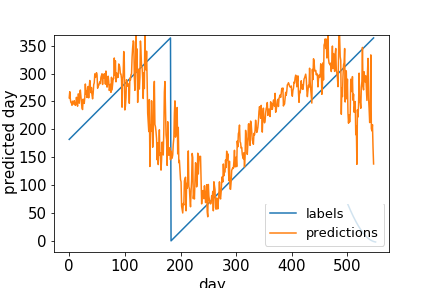
\includegraphics[width=0.5\linewidth]{figures/global_linear_results.png}
    \caption{Global regression with linear representation}
    \label{fig:glob_linear}
\end{figure}

The predictions seem to have a smoother periodic response, so the representation may be at fault. Indeed, using Mean squared error loss and a non continuous function as label is not compatible. The parameters for day 0 and day 365 are very similar as they are both in winter, but the loss will be maximal if there is an error between them, while the true error is only very small.

\paragraph*{}
Otherwise, using a cosine representation ($\textrm{day} = (\cos{2\pi\textrm{D}/366}+1)/2$) produce better results, with $\textrm{MSE} = 0.05, \textrm{MAE} = 0.05, \textrm{R2} = 0.9686$. The prediction can be observed in Fig. \ref{fig:glob_cos}. The problem with this representation is that it is impossible to differentiate Spring days from Autumn days.

Using only the polynomial of order 0, the results are $\textrm{MSE} = 0.10, \textrm{MAE} = 0.10, \textrm{R2} = 0.8817$. Again, the same trend is observed and the CNN performs better than learning only on the time series.

\begin{figure}[!ht]
    \centering
    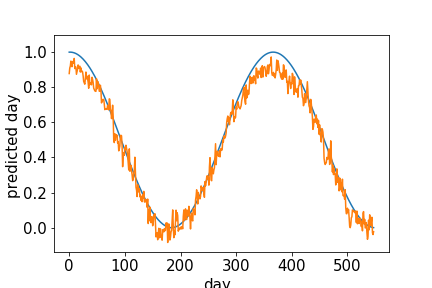
\includegraphics[width=0.5\linewidth]{figures/global_cos_results.png}
    \caption{Global regression with cosine representation}
    \label{fig:glob_cos}
\end{figure}

As seen in Figure \ref{fig:evol_temp}, the temperature is already a function of the time similar to a sine. To make the problem harder, only the precipitation feature is used for the next experiment, as its correlation with time is not easily understandable by a human (Fig. \ref{fig:prec_time}).

\begin{figure}[!ht]
    \centering
    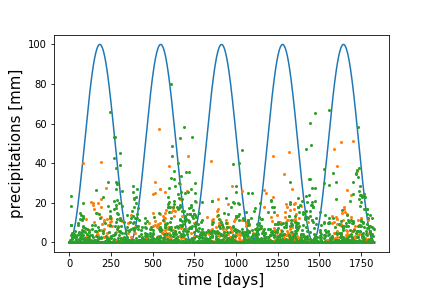
\includegraphics[width=0.5\linewidth]{figures/prec_time.png}
    \caption{Precipitation for two stations\\Blue cosine is the evolution of the years}
    \label{fig:prec_time}
\end{figure}

\paragraph*{}
The result is not as smooth as with the temperature as input feature, but the behaviour is still the same. With a filter of order 0, the model behaves poorly. The metrics are: $\textrm{MSE} = 0.58, \textrm{MAE} = 0.42, \textrm{R2} = -0.98$. Without any surprise at this point, having a convolution with an order K=5 increases the performance, and the metrics are better: $\textrm{MSE} = 0.50, \textrm{MAE} = 0.18, \textrm{R2} = 0.5971$ and the prediction is shown in Fig. \ref{fig:glob_prec}. Even if the result is better than the performance of the filter of order 0, it is still far from ideal and cannot be called a complete success.

\begin{figure}[!ht]
    \centering
    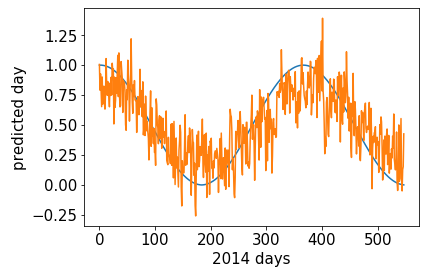
\includegraphics[width=0.5\linewidth]{figures/global_cos_reg_results.png}
    \caption{Global regression using only precipitation feature}
    \label{fig:glob_prec}
\end{figure}

\subsection{Further improvement}
\paragraph*{}
One possibility to improve the results, even if there is little hope to do that, and an interesting thing to do, is to add pooling, and use an auto-encoder decoder architecture. An exploration of different methods for irregular graph pooling is in appendix \ref{sec:irreg_pool}. 

Another possibility is to perform convolution on the time axis. In practice, the graphs can be multiplied by a Kronecker product for each day.

\paragraph*{}
Another interesting approach that has not yet been tried, is to use only station related and time related features, and do the regression to find the measurements. The model will then learn descriptors for the weather stations and find relations between them such as climate type.



\section{Climate event detection - ExtremeWeather}\label{task:ExtremeWeather}
\paragraph*{}
At the time of writing, the experiments were still running, so no results can be presented.
\subsection{Task presentation}
\paragraph*{}
The ExtremeWeather dataset \cite{racah_extremeweather:_2017} is composed of 4 measurements per day, 365 days per year (no extra measurement for leap years). All measurements have 16 different channels corresponding to a different feature, and the world is represented by an equiangular grid of 768 by 1152 pixels, which results in a total of approximately 885k pixels.

For their climate pattern segmentation problem, Jiang and Cohen used a tessellation of an icosahedron of order 5, having $10\cdot4^5+2 = 10'242$ pixels using bilinear interpolation. Inspired by them, a HEALPix map is used using bilinear interpolation on the latitude, longitude grid, with a density $N_{side}$ of 32.

\begin{figure}[!ht]
    \centering
    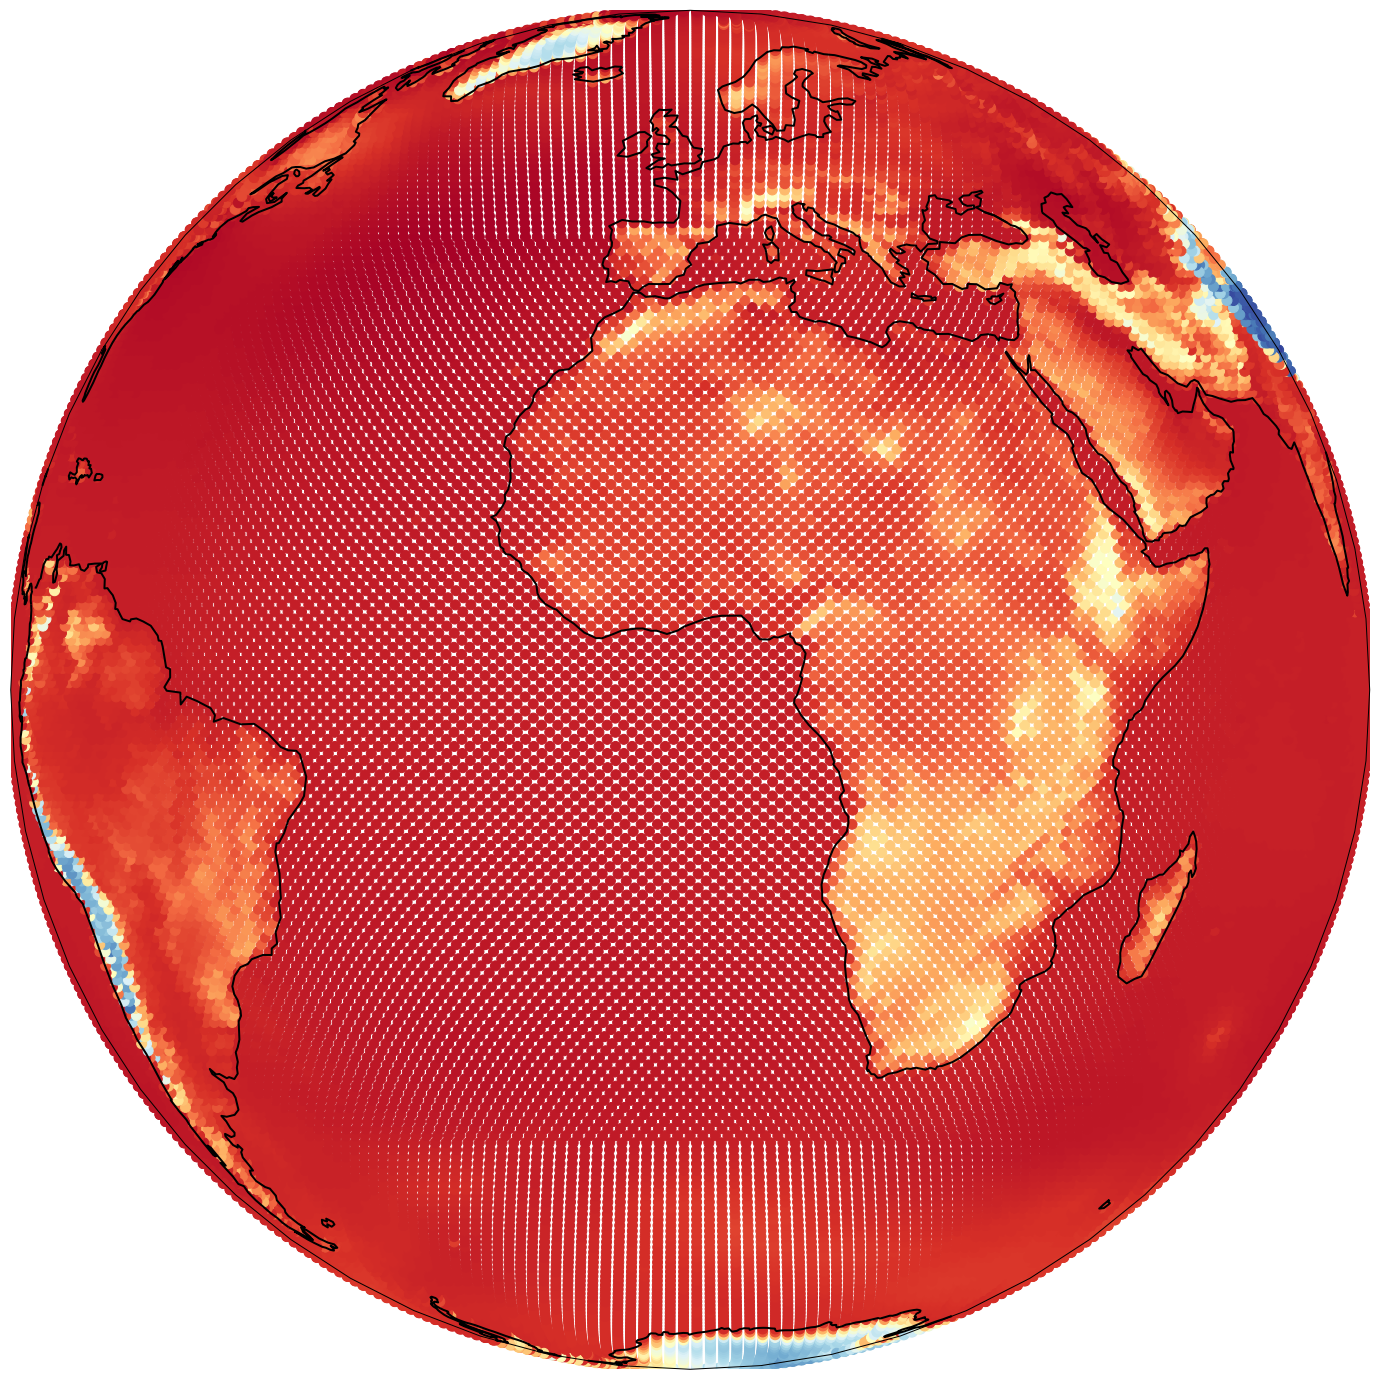
\includegraphics[width=0.6\linewidth]{world_nside32.png}
    \caption{Bilinear interpolation of Atmospheric Pressure at sea level at $N_{side}=32$}
    \label{fig:EW_nside32}
\end{figure}

Concerning the labels, only the bounding boxes are given. Before creating the groundtruth accurately, all pixels inside bounding box is considered belonging to the corresponding class.
\subsection{Implementation}
\paragraph*{}
As an HEALPix map is used, average pooling can be used, and an architecture similar to U-NET\cite{ronneberger_u-net:_2015} is built.

\paragraph*{}
The deconvolution, the transpose convolution, is exactly the same graph convolution used by DeepSphere. Additionally, it is easier to use average pooling than max pooling in order to do the unpooling.


% \subsection{our model and result}
% \subsection{conclusion}
\section{Climate pattern segmentation}\label{task:climate}
\paragraph*{}
This section is still incomplete as the dataset is still not public at the time of the writing of the report. This will hopefully be completed at a later time.

\subsection{Task presentation}
\paragraph*{}
Other spherical CNNs have already run this experiment but with another sampling, based on the icosahedron. The sCNNs are made by Jiang \cite{jiang_spherical_2019} and Cohen \cite{cohen_gauge_2019}. 
% \paragraph*{}
% The dataset is accessible at \url{https://portal.nersc.gov/project/dasrepo/deepcam/segm_h5_v3_reformat/}. Acknowledge good people

% Read me at \url{https://portal.nersc.gov/project/dasrepo/deepcam/segm_h5_v3_reformat/gb_data_readme}
% \todo[inline]{finish this subsection.}

% \section{Prove flexibility dataset}
% \todo[inline]{future work to do. No time for experiments}
% \subsection{dataset and task}
% \subsection{our approach}




\chapter{Conclusion}
\section{Synthesis}
\paragraph*{}
In this section, the conclusions from all the tasks will be summed up in order to conclude on the differences and potential advantages of DeepSphere. In other words, we analyze how well our model competes against other state-of-the-art spherical CNNs.

\paragraph*{}
Concerning the speed of the computation, and thus of the learning time, it was principally measured in the section \ref{task:shrec17}, during the shape retrieval task. Thus, DeepSphere runs 4 to 40 times faster than other spherical CNNs using Fourier transform to reach peak performance, and an inference time 10 times faster with a small local filter.
% \todo[inline]{If time, compute Jiang time too, and MoNet}

Furthermore, SHFT-SCNNs are not able to run the learning of the cosmological maps classification in an acceptable time (section \ref{task:cosmo}).
% \todo{run cohen and esteves with cosmo maps}

\paragraph*{}
Furthermore, the flexibility of DeepSphere is proven with the regression task in section \ref{task:GHCN}. Using an irregular sampling of the sphere is not doable by spherical CNNs using Fourier transform or planar projection, unless one interpolates it into another sampling. Additionally, it is shown that having an idea of the locality increases the performance, rather than working only on the time series of each nodes. Thus using a CNN makes indeed more sense.

\paragraph*{}
Regarding the shape retrieval and shape classification task, in sections \ref{task:shrec17} and \ref{task:mn40}, the obtained results were similar to the results of the other models, even though lower for ModelNet40. Thus it can be safely stated that equivariance to the third rotation of $SO(3)$ is an unnecessary price to pay. 
% \todo{Maybe it is possible to have better results on MN40 with a different architecture}

\paragraph*{}
Concerning the approximation of the spherical harmonics with the eigenvectors of the Laplacian of the HEALPix graph, leading to an almost equivariant to rotation convolution, it is shown during the SHREC17 task that using a theoretically better graph  does not lead to better results. This is mostly due to the fact that the important information lies in the low frequency. And this explains why the model still performs well with a poor sampling resolution ($N_{side}=8$).
Again, using a better graph did not lead to a better result for the ModelNet40 task. Thus, it can be safely stated that the model is sufficiently equivariant to rotation for the considered tasks.

For the regression task, and for the not experimented segmentation task, there is no indication that equivariance to rotation helps. %It would rather be the contrary.

\paragraph*{}
The other tasks not presented (segmentation and object detection on weather data) were chosen to show different uses of DeepSphere and illustrate the multiple applications it can have.

\paragraph*{}
Finally, DeepSphere is not able to outperform the state of the art on established tasks, but can reach similar results in a shorter time.

\section{Future Work}
\paragraph*{}
As there are some tasks still in suspense, the first thing to do is to complete them. Concerned tasks are (1) the climate pattern segmentation in section \ref{task:climate} and (2) the climate event detection in section \ref{task:ExtremeWeather}.

\paragraph*{}
Another task that would have been nice to have is a scene classification or segmentation, to have another point of comparison with \cite{cohen_gauge_2019} and \cite{jiang_spherical_2019}. That would also allow to work on a different kind of data, omnidirectional images, where equivariance to rotation is not necessary a good thing to have, like an isotropic filter. Indeed, some objects in these images are often linked with another one in a fixed configuration, and an anisotropic filter may capture this information.

\paragraph*{}
Again, an intensive analysis of speed versus performance of different configurations of DeepSphere would have been great, and should be done in a future work.

\paragraph*{}
Finally, going out of the scope of this study, other symmetries could be explored and easily reached with another graph. For example, in the case of omnidirectional imaging, and more specifically, panoramas, the images are always oriented with the gravity. 

On another note, in this example, a cylinder could be a better graph, as the axis of the cylinder corresponds to the gravity's orientation, and the angle to the rotation of the panoramic point of view. %Only missing symmetries would be local rotation.

It would be possible to create a dataset from panoramas of cameras, having only a 360\degree (or less) on view with the same pitch, and could be use as a proof of concept.


\section*{Acknowledgements}
\emph{I would like to thank Carlos Esteves for helping understanding his code and providing assistance for the SHREC17 task, and Chiyu "Max" Jiang and Steve Farrell for providing access to climate data for the climate pattern segmentation task.
Finally, I would like to thank Michaël Defferard and Nathanaël Parraudin for their help and guidance throughout this project, as well as Martino Milani, Charles Gallay and Luca Zampieri with whom I enjoyed worked with and whose valuable advice and insight I appreciated.}

\printbibliography
\addcontentsline{toc}{chapter}{Bibliography}
\cleardoublepage
\mbox{~}
\cleardoublepage
\appendix
\chapter{Miscellaneous}
\section*{Improving DeepSphere implementation}
\paragraph*{}
The original version of DeepSphere was implemented with python using TensorFlow\footnote{\url{https://www.tensorflow.org/}} (TF). As it was using an old way to transfer the data to the GPU, some modifications were necessary for the experiments of this project. Indeed, the shape retrieval task deals with a great amount of data, and the whole dataset cannot be loaded in the RAM at the same time, especially when augmentation is used and different perturbed versions of the same instance exist.
The old way is refered as "Dataset load on RAM" as it consisted in loading the whole data directly on the RAM, and transferring it to the GPU batch by batch.

\paragraph*{}
The code for the experiment is based on Cohen's work\footnote{\url{https://github.com/jonas-koehler/s2cnn/tree/master/examples/shrec17}}, and was using npy files\footnote{\url{https://www.numpy.org/devdocs/reference/generated/numpy.lib.format.html}} to store the preprocessed data. The intermediate solution consisting in reading the files when needed is called "Dataset loaded on the fly".

To reduce the unwanted idle time between each batch, the TF dataset pipeline is used. 

It was only later discovered that the dataset pipeline handling is optimized with the use of TFrecords files to store the preprocessed data. The amount of work necessary to rebuild the dataset was deemed too much and the improvements unnecessary.

\paragraph*{}
The performance of each setting is tested on the architecture \emph{Cohen-like}, with 20 epochs and an evaluation of a validation set using the method "Dataset loaded on RAM" every 0.5 epoch.
\paragraph*{}
\begin{tabular}{|c|c|c|c|c|}
\hline
~ & Time per batch & CPU time & Wall time  & Load average  \\ \hline
\begin{tabular}{c}
Dataset loaded\\
on RAM
\end{tabular}
 & 0.12 s & 1598 s & 2693 s & 80\% \\ \hline
\begin{tabular}{c}
Dataset loaded\\
on the fly
\end{tabular}
 & 
\begin{tabular}{c}
0.11 +   \\
0.06 s\\(loading time)
\end{tabular}
& 2541 s & 3667 s  & 50\% \\ \hline
TF Dataset pipeline & 0.09 s & 2400 s & 2046 s & 90\% \\ \hline
% \begin{tabular}{c}
% TF Dataset\\
% pipeline w/ TFRecords
% \end{tabular}
%  & 
% \multicolumn{4}{c|}{TODO in the future to further improve performance} \\ \hline
\end{tabular}

\section*{Inference time analysis}
\paragraph*{}
A quick analysis of the inference time of the architecture \emph{Cohen-like} is performed on the shape retrieval task in order to see the influence of the HEALPix graph (in function of the $N_{side}$ parameter) and the size of the filter $K$. The batch size is 32.

\paragraph*{}
\begin{table}[]
    \centering
    \begin{tabular}{|c|ccc|} \hline
        $N_{side}$  & 32 & 64 & 128 \\
        Batch time [s]  & 0.07 & 0.26 & 1.15\\\hline 
        \multicolumn{4}{c}{}\\\hline
        K    & 2 & 4 & 5 \\
        Batch time [s] & 0.11 & 0.19 & 0.26 \\\hline
    \end{tabular}
    \caption{Evolution of inference time}
    \label{tab:app_infer_time}
\end{table}

\paragraph*{}
The evolution of the time is then linear in function of $K$ and the number of pixels ($12\cdot N_{side}^2$

\chapter{Pooling non-uniform graph}\label{sec:irreg_pool}
\paragraph*{}
One of the problem with a graph built from a non-uniform sampling is that the pooling operation is non-trivial since the sampling is not hierarchical.

Thus, different pooling methods are explored for this graph.

\begin{figure}[!ht]
    \centering
    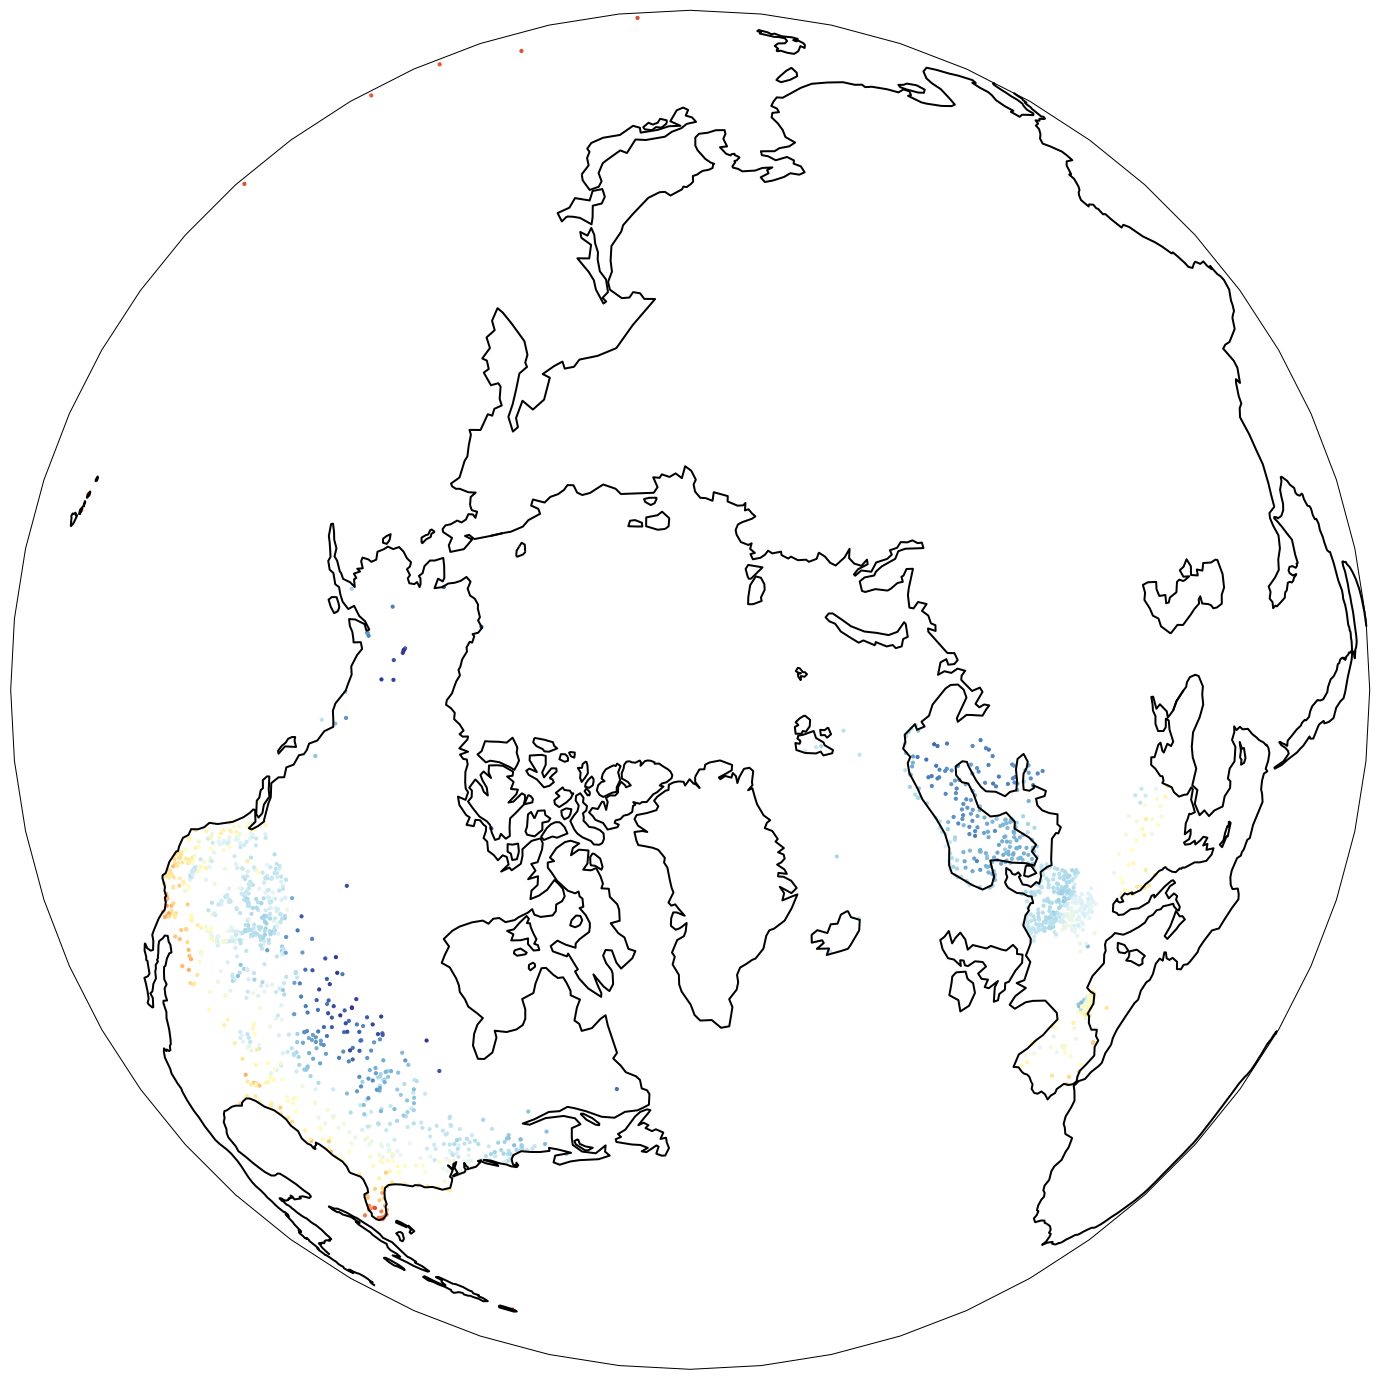
\includegraphics[width=0.6\linewidth]{figures/original_signal.png}
    \caption{Original signal on non-uniform sampling\\low values are represented in blue and high values in red}
    \label{fig:origin_sig}
\end{figure}
\clearpage
\paragraph*{}
A first one consists to using a hierarchical sampling with less pixels and interpolating the signals. An example is made from the popular HEALPix. A $N_{side}$ is chosen such that the number of pixels is inferior than the number of nodes from the graph. The four HEALPix pixels closest to each node are chosen, and their value is computed from the original pixel.

\begin{figure}[!ht]
    \centering
    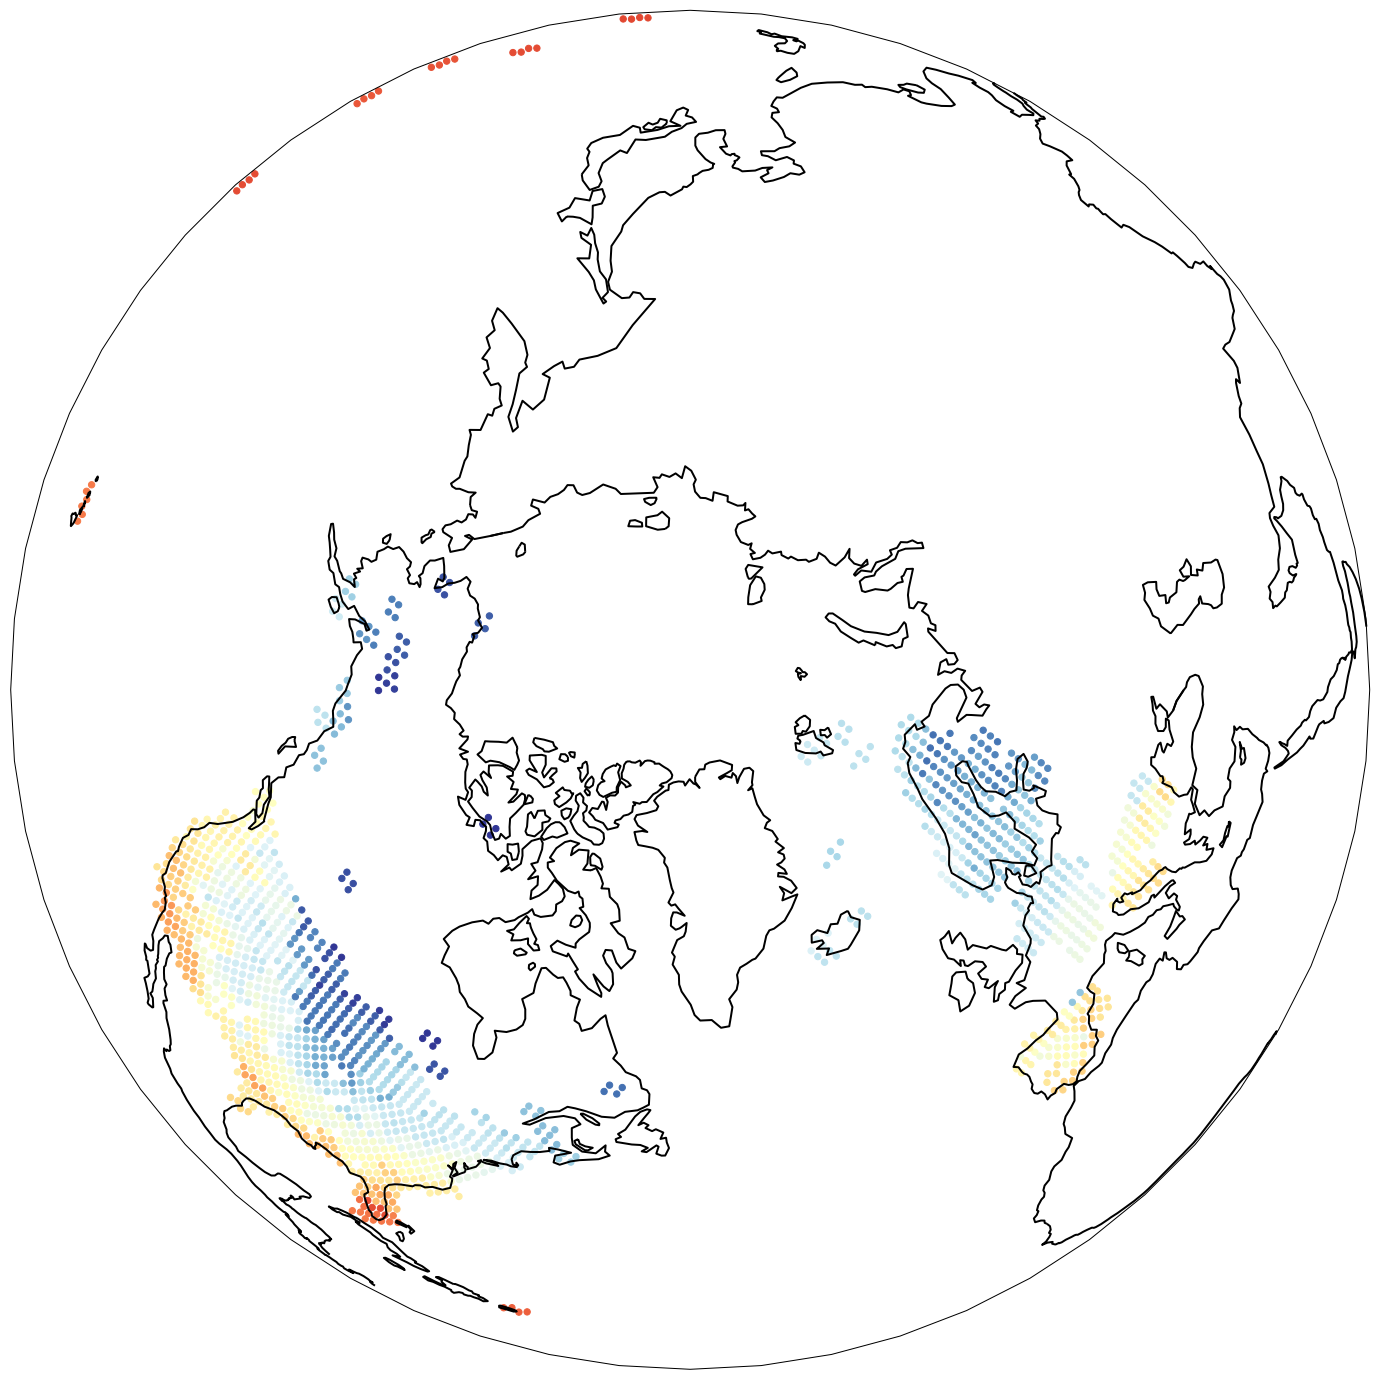
\includegraphics[width=0.6\linewidth]{figures/healpix_pool_signal.png}
    \caption{Pooled signal to HEALPix sampling}
    \label{fig:pool_healpix}
\end{figure}
\clearpage
\paragraph*{}
A second one consists to carry out a spectral clustering of the graph using a number of cluster corresponding to the desired number of pixels after the pooling operation. The goal of this method is to keep the pseudo-structure of the previous graph.

Practically, KMeans is applied on the eigenvectors of the combinatorial Laplacian to identify the clusters, and new pixels are the center of these clusters.

The main problem with this method is the treatment of far isolated pixels. If these kind of pixels is clustered with other pixels far from it, the resulting cluster will hold no sense.

\begin{figure}[!ht]
    \centering
    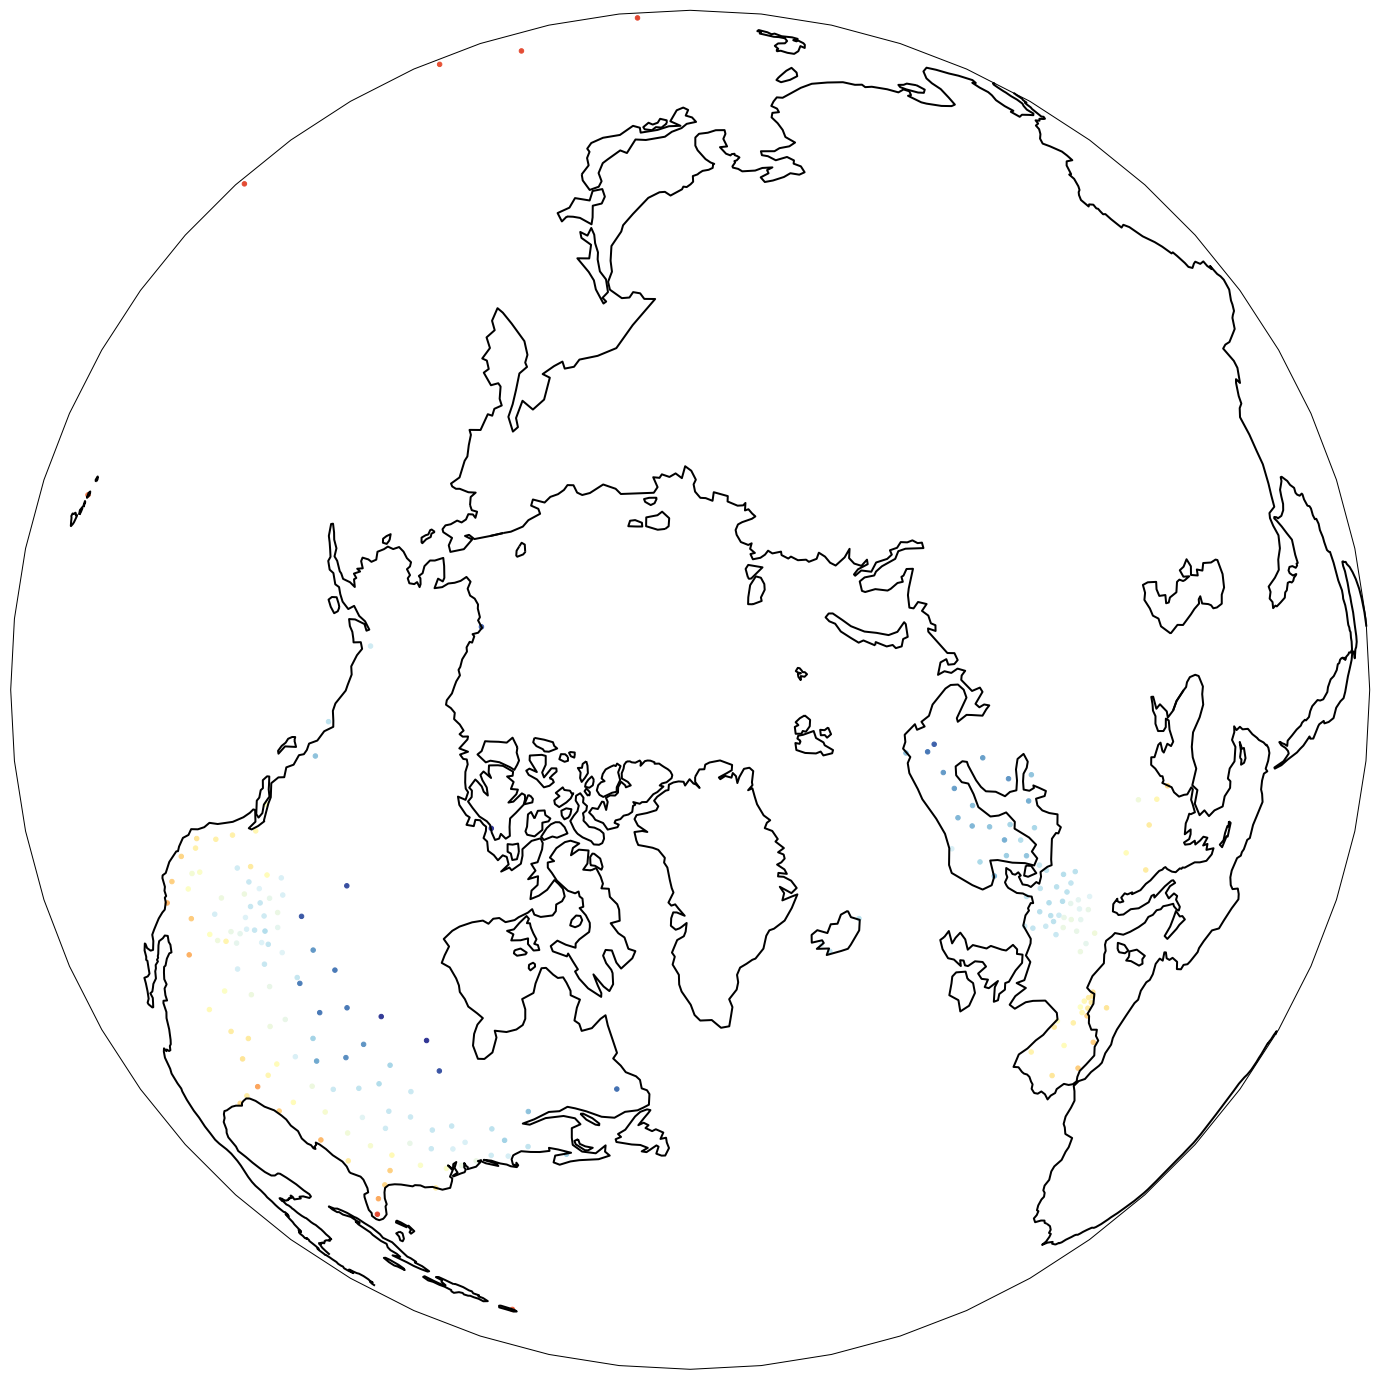
\includegraphics[width=0.6\linewidth]{figures/cluster_pool_signal.png}
    \caption{Pooled signal to clusters}
    \label{fig:pool_cluster}
\end{figure}

\paragraph*{}
Finally, a more general method will be to sparsify the graph, thus removing nodes that are not important. The methods implemented on PyGSP\footnote{\url{https://pygsp.readthedocs.io/en/stable/reference/reduction.html}} are tried, but do not give satisfying results as the resulting graph loses its coordinates.

\paragraph*{}
As it was just an exploration of possible methods, no implementation in TensorFlow was done to exploit them.
% \chapter{MoNet comparison}

% use of pytorch geometric to do the experiments.

% for each conv layer, give nfeatin, nfeatout, dim, Ksize, aggr, rootweight, bias
% dim=1 because the pseudo-coordinates in the case of DeepSphere is only the weighted edge between two nodes.
\end{document}